%%%%%%%%%%%%%%%%%%%%%%%%%%%%%%%%%%%%%%%%%%%%%%%%%%%%%%%%%%%%%%%%%%
%                                                                 %
%   KUIP  - Reference Manual -- LaTeX Source                      %
%                                                                 %
%   Chapter 2: User Interface                                     %
%                                                                 %
%   External EPS files referenced: styles.eps, styleg.eps         %
%                                  stylegp.eps, stylem.eps,       %
%                                  tree.eps                       %
%                                                                 %
%   Editor: Michel Goossens / CN-AS                               %
%   Last Mod.: 10 Dec  1992   mg                                  %
%                                                                 %
%%%%%%%%%%%%%%%%%%%%%%%%%%%%%%%%%%%%%%%%%%%%%%%%%%%%%%%%%%%%%%%%%%%

\newif\ifVECTOR \VECTORfalse % describe get vector stuff ?

\ifPAWman
\VECTORtrue
\def\PROMPT{\Lit{PAW >}}
\fi
\ifKUIPman
\VECTORtrue
\def\PROMPT{\Lit{KUIP >}}
\fi

\ifKUIPman

\chapter{User interface}
%
%---------------------------------------------------------------------------
%
\section{Dialogue Styles}

In a \KUIP{}-based application the user has the choice of
different dialogue styles ranging from the conventional command line
interface to a high-level windowed environment based on \OSFMotif{}.
The optimum choice for each user depends on the level of experience
and also on the type of terminal or workstation available.
The user can freely switch between the different styles from within
the application using the command \Cind{STYLE}.
The only exception is the \Motif{} interface since its internal structure
is completely different from the others.

Underneath of all these different dialogue style lies a common
processing engine.
The command and its arguments is extracted from the input which was
either typed in directly by the user or constructed by one of the menu
styles and then the appropriate application routine is called.
Even when using a menu-driven style a basic knowledge of the command
processing is necessary, e.g.\ how commands can be abbreviated and what is the
meaning of special characters.
Before plunging into the details of the command syntax we want to
overview the capabilities of the individual styles.


\subsection{Alphanumeric modes}

The styles ``\Lit{C}'', ``\Lit{AN}'', and ``\Lit{AL}'' can be
used with any kind of terminal device.

\subsubsection{STYLE C}

\Lit{STYLE C} is the basic keyboard input mode:
the user types a command line which is then executed.
After being more familiar with the command set of an application, most
users actually prefer \Lit{STYLE C} to type in everything to avoid
the frequent switching between mouse and keyboard input required by
graphical menu techniques.

\KUIP{} provides an integrated online help facility.
The first line to type in an unfamiliar application is
``\Lit{HELP}'' (or ``\Lit{help}'' --- \KUIP{} command names are
case-insensitive) which shows the top level of the command tree.
Taking \PAW{} as one of the prime examples of a \KUIP{}-based
application we get the following output:
\begin{XMP}
PAW > \underline{help}

From  /...

 1:   KUIP          Command Processor commands.
 2:   MACRO         Macro Processor commands.
 3:   VECTOR        Vector Processor commands.
 4:   HISTOGRAM     Manipulation of histograms, Ntuples.
 5:   FUNCTION      Operations with Functions. Creation and plotting.
 6:   NTUPLE        Ntuple creation and related operations.
 7:   GRAPHICS      Interface to the graphics packages HPLOT and HIGZ.
 8:   PICTURE       Creation and manipulation of HIGZ pictures.
 9:   ZEBRA         Interfaces to the ZEBRA RZ, FZ and DZ packages.
10:   FORTRAN       Interface to MINUIT, COMIS, SIGMA and FORTRAN Input/Output.
11:   NETWORK       To access files on remote computers.
12:   OBSOLETE      Obsolete commands.

Enter a number ('Q'=command mode):
\end{XMP}

At this point we can either enter ``\Lit{Q}'' to return to the
command line prompt again, or we can investigate the command tree.
Typing ``\Lit{1}'' show us the commands and sub-menus which are linked
to the menu ``\Lit{/KUIP}'':
\begin{XMP}
Enter a number ('Q'=command mode): \underline{1}

   /KUIP

   Command Processor commands.

From  /KUIP/...

 1: * HELP          Give the help of a command.
 2: * USAGE         Give the syntax of a command.
 3: * MANUAL        Write on a file the text formatted help of a command.
 4: * EDIT          Invoke the editor on the file.
 5: * PRINT         Send a file to the printer.
 6: * PSVIEW        Invoke the PostScript viewer on the file.
 7: * LAST          Perform various operations with the history file.
 8: * MESSAGE       Write a message string on the terminal.
 9: * SHELL         Execute a command of the host operating system.
10: * WAIT          Make a pause (e.g. inside a macro).
11: * IDLE          Execute a command if program is idle.
12: * UNITS         List all Input/Output logical units currently open.
13: * EXIT          End of the interactive session.
14: * QUIT          End of the interactive session.
15:   FUNCTIONS            *** KUIP System Functions ***
16:   ALIAS         Operations with aliases.
17:   SET_SHOW      Set or show various KUIP parameters and options.

Enter a number ('\bsol'=one level back, 'Q'=command mode):
\end{XMP}

The menus \Lit{/KUIP} and \Lit{/MACRO} contain the \KUIP{}
built-in commands which are common to all applications.
Now we could continue wandering around the command tree by choosing
one of the sub-menus or by entering ``\bsol'' to go back to the previous menu.
Instead we can also select one of the actual commands which are marked
by ``\Lit{*}'':
\begin{XMP}
Enter a number ('\bsol'=one level back, 'Q'=command mode): \underline{1}

 * KUIP/HELP [ ITEM OPTION ]

   ITEM       C 'Command or menu path' D=' '
   OPTION     C 'View mode' D='N'

   Possible OPTION values are:

    EDIT    The help text is written to a file and the editor is invoked,
    E       Same as 'EDIT'.
    NOEDIT  The help text is output on the terminal output.
    N       Same as 'NOEDIT'

   Give the help of a command.  If ITEM is a command its full explanation is
   given:  syntax (as given by the command USAGE), functionality, list of
   parameters with their attributes (prompt, type, default, range, etc.).  If
   ITEM='/' the help for all commands is given.

   If HELP is entered without parameters or ITEM is a sub-menu, the dialogue
   style is switched to 'AN', guiding the user in traversing the tree command
   structure.

   'HELP -EDIT' (or just 'HELP -E') switches to edit mode:  instead of writing
   the help text to the terminal output, it is written into a temporary file
   and the pager or editor defined by the command HOST_PAGER is invoked.  (On
   Unix workstations the pager can be defined to display the help text
   asynchronously in a separated window.) 'HELP -NOEDIT' (or just 'HELP -N')
   switches back to standard mode.  The startup value is system dependent.

<CR>=continue, 'Q'=command mode, 'X'=execute:
\end{XMP}

Here we see the help text for the \Cind{HELP} command itself.
In fact the command is not called ``\Lit{HELP}'' but
``\Lit{/KUIP/HELP}'' and has two parameters.
Nevertheless \KUIP{} recognized the abbreviation and provided
default arguments (``\Lit{D=...}'') which allowed the command to be
executed. 

Typing ``\Lit{X}'' allows to execute the current command
--- for the \Cind{HELP} command itself this would not be very useful.
Simply hitting the \textsc{RETURN} or \textsc{ENTER}-key would
brings us back to the previous menu.
Instead we want to use ``\Lit{Q}'' which brings us back to the
command line mode.

As we have seen the \Cind{HELP} command actually can take two arguments.
The second one we ignore for the moment since the first one is much more
important.
If we know the name of a command but do not know what it is doing
exactly we can get the help text directly without going through the help
menu mode:
\begin{XMP}
PAW > \underline{help usage}

 * KUIP/USAGE ITEM

   ITEM       C 'Command name'

   Give the syntax of a command.  If ITEM='/' the syntax of all commands is
   given.
\end{XMP}

The command \Cind{USAGE} is also part of the online help system.
It shows the first line only of the help information in case we know what a
command is supposed to do but are not sure about the number and order or
arguments:
\condbreak{4\baselineskip}
\begin{XMP}
PAW > \underline{usage manual}

 * KUIP/MANUAL ITEM [ OUTPUT OPTION ]
\end{XMP}
This tells us that the \Cind{MANUAL} command takes three arguments of
which the last two are optional.
Although we do not know yet what this command is doing we try it
nevertheless:
\begin{XMP}
PAW > \underline{manual}
Command or menu path (<CR>=manual)

 * KUIP/MANUAL ITEM [ OUTPUT OPTION ]

   ITEM       C 'Command or menu path'
   OUTPUT     C 'Output file name' D=' '
   OPTION     C 'Text formatting system' D=' '

   Possible OPTION values are:

   ' '     plain text : plain text format
    LATEX  LaTeX format (encapsulated)
    TEX    LaTeX format (without header)

   Write on a file the text formatted help of a command.  If ITEM is a menu 
   path the help for all commands linked to that menu is written.  If ITEM='/' 
   the help for the complete command tree is written.  If OUTPUT=' ' the text 
   is written to the terminal.  

   The output file produced with option LATEX can be processed directly by 
   LaTeX, i.e. it contains a standard header defining the meta commands used 
   for formatting the document body.  With option TEX only the document body 
   is written into the output file which can be included by a driver file 
   containing customized definitions of the standard meta commands.  Example:  

    MANUAL / MAN.TEX LATEX

   will produce the file MAN.TEX containing the documentation of all available 
   commands in LaTeX format.  
\end{XMP}

\KUIP{} realized that we did not give any argument.
Since the first parameter \Pind{ITEM} is mandatory the command cannot be
executed without one.
We were prompted for it and accepted the proposed default value.
(It is a peculiarity of the \Cind{MANUAL} command that the default
depends on the preceding \Cind{HELP}, \Cind{USAGE}, or \Cind{MANUAL}
command. 
Usually it is either a value fixed by the application writer or the one
used in the previous execution of the very same command.)

The output of this \Cind{MANUAL} command looks exactly the same as for
the corresponding \Cind{HELP} command.
The behavior becomes different, however, when \Pind{ITEM} is not a
command but a menu name.
``\Lit{HELP KUIP}'' enters the help menu mode starting off at the
\Lit{/KUIP} menu instead of the root menu ``\Lit{/}''.
``\Lit{MANUAL KUIP}'' on the other hand shows the help text for all
commands linked to this menu and all of its sub-menus.
Furthermore the output can be redirected into a file and beefed up with
\LaTeX{} formatting directives.


\subsubsection{STYLE AN}

\Lit{STYLE AN} is very similar to the help menu mode in 
\Lit{STYLE C}.
The only difference is that when selecting a command the question
\begin{XMP}
<CR>=continue, 'Q'=command mode, 'X'=execute:
\end{XMP}
is never asked.

\subsubsection{STYLE AL}

\Lit{STYLE AL} is a slight variation of \Lit{STYLE AN} using
letters instead of numbers to label the items:
\begin{XMP}
PAW > \underline{style al}

From  /...

 A:   KUIP          Command Processor commands.
 B:   MACRO         Macro Processor commands.
 C:   VECTOR        Vector Processor commands.
 D:   HISTOGRAM     Manipulation of histograms, Ntuples.
 E:   FUNCTION      Operations with Functions. Creation and plotting.
 F:   NTUPLE        Ntuple creation and related operations.
 G:   GRAPHICS      Interface to the graphics packages HPLOT and HIGZ.
 H:   PICTURE       Creation and manipulation of HIGZ pictures.
 I:   ZEBRA         Interfaces to the ZEBRA RZ, FZ and DZ packages.
 J:   FORTRAN       Interface to MINUIT, COMIS, SIGMA and FORTRAN Input/Output.
 K:   NETWORK       To access files on remote computers.
 L:   OBSOLETE      Obsolete commands.

Enter a letter ('Q'=command mode): 
\end{XMP}


\subsection{Graphics modes}

The graphics styles \Lit{G} and \Lit{GP} can only be used on
workstations.
Furthermore they are only operational if the application writer has
chosen to do so. 
(The \KUIP{} main loop has to be invoked by calling \Rind{KUWHAG}
instead of \Rind{KUWHAT}.
This implies to link the application with the graphics library
(e.g.\ \Lit{GRAFX11} or \Lit{GRAFGPR}) containing the appropriate
\HIGZ{} version for the underlying windowing system. 

\begin{figure}[tb]
\begin{center}
\mbox{\epsfig{file=styleg.eps,width=.8\textwidth}}
\end{center}
\caption{Example of STYLE G}
\label{FIG4}
\end{figure}

The user interacts with the application by moving the mouse pointer to
appropriate box and clicking with the left mouse button.
If the corresponding action requires additional keyboard input the mouse
pointer changes into a question mark shape.
Pressing the right mouse button leaves the graphics mode and reverts to
style~\Lit{C}.

The style names \Lit{G} and \Lit{GP} allow additional attributes
\Lit{S} and \Lit{W} which may also be combined, e.g.\
\Lit{GSW}.
The attribute \Lit{S} uses software characters for writing texts in
case the hardware font does not have the right size.
The attribute \Lit{W} uses a shadow width effect to give a 3D impression.


\subsubsection{STYLE G}

\Lit{STYLE G} is similar to \Lit{STYLE AN} but the
menus are displayed in the graphics area (see figure~\ref{FIG4}).
This restricts the part of the graphics window available for other
graphics output to the shaded area.
The actual size of the reserved area can be adjusted by additional arguments
to the \Cind{STYLE} command.

Menus are marked by black vertical bars and the presently active menu
levels are high-lighted.
When finally a command name is selected the panel displayed in the top
left corner shows the parameter descriptions and allows to set argument
values and execute the command.


\subsubsection{STYLE GP}

\Lit{STYLE GP} displays a user-defined panel in the top part of the
graphics area (see figure~\ref{FIG5}).
The layout and content of the panel is defined by the \Cind{PANEL}
command.
(Actually, if a panel is defined it is also displayed by
style~\Lit{G}.
Therefore style~\Lit{GP} has to be read as ``panel-only'' rather
than ``panel'' style.)
 
\begin{figure}[tb]
\begin{center}
\mbox{\epsfig{file=stylegp.eps,width=.8\textwidth}}
\end{center}
\caption{Example of STYLE GP}
\label{FIG5}
\end{figure}

The content of each panel box gives the command which is executed when
clicked on it.
Some characters have a special meaning in the panel command sequences:
\begin{XMP}
panel 0
panel 1 Edit-     Exec- Shell-     Vector/List  Alias/List -     HELP-   EXIT
panel 2 'Ldir //' Cdir- Histo/List Histo/Plot-  Histo/Plot Lego  Surface Contour
panel 3 Set-      Opt-  Igset-     ' '          Locate     Zone- Next    Null
panel 4 'Histo/Plot $ E | Plot error bars'      'Exec paneldoc--'
\end{XMP}
Everything following ``\Lit{|}'' is ignored.
``\Lit{$}'' requests and is replaced by keyboard input.
A single ``\Lit{-}'' at the end of the command sequence is replaced
by the keyboard input separated by a blank.
(This minimizes the need for quotes in the \Cind{PANEL} command, e.g.\
``\Lit{Edit-}'' instead of ``\Lit{'Edit $'}''.)
The blank separation is suppressed if the command ends with ``\Lit{--}''.

Style \Lit{GP} is very useful for applications where a limited set
of commands has to be executed frequently, for example in an online monitoring
package or in an event display program.
The panel definition and the switch to style \Lit{GP} could actually
be contained in file which is executed at startup time.
Whilst being in style~\Lit{GP} the panel can also be redefined.
For example, clicking on ``\Lit{Exec paneldoc--}'' and entering
``\Lit{1}'' executes the macro file \Lit{paneldoc1.kumac} which
could contain:
\begin{XMP}
panel 0
panel 1 'Histo/Plot 1' 'Histo/Plot 2' 'Histo/Plot 3' 'Histo/Plot 4'
panel 2 'Histo/Plot 5' 'Histo/Plot 6' 'Histo/Plot 7' 'Histo/Plot 8'
panel 3 'Cdir //LUN1' 'Cdir //LUN2'
panel 4 'Exec paneldoc | to go back'
\end{XMP}
%
%
\subsubsection{STYLE XM}

MOTIF is not a ``\KUIP{} STYLE'' in the same sense as ``STYLE G'' or ``STYLE GP''.
When an application has decided to use \KUIPMotif{} switching to another
style is not possible. This is not a real drawback in the sense that
all the features provided by the other styles are included in \KUIPMotif{} 
(e.g.\ command mode and panel(s) handling).

\begin{figure}[tb]
\vspace{-.5cm}
\PICT{pkmf1}
\vspace{-1cm}
\caption{What Do You Get ?}
\label{ref:FIGPKMF1}
\vspace{-.5cm}
\begin{EnumZB}
\item \EW{}
\item \MB{}.
\item HIGZ \GW{} (optional).
\item User definable panel of commands (\PNI{}).
\end{EnumZB}
\begin{EnumZW}
\item \MB{} entry for ``Commands''.
\item Pulldown Menu`` Commands''.
\item \INP{}.
\end{EnumZW}
\vspace{-.5cm}
\vspace{10pt}
\end{figure}

\begin{figure}[tb]
\PICT{pkmf2}
\caption{Pulldown Menu Access to Commands}
\label{ref:FIGPKMF2}
\begin{EnumZB}
\item Pulldown menu ``Commands'' with the complete tree command structure.
\item \CAP{} for the \KUIP{} command /KUIP/SET\_SHOW/STYLE.
\end{EnumZB}
\end{figure}


An application based on \KUIPMotif{} will always start 2 processes, which
will give at least 2 windows (Fig. \ref{ref:FIGPKMF1}):
\begin{UL}
\item
The \EW{} \NbDB{1} is a terminal emulator built in inside \KUIP{}. It 
enables a powerful ``command input and output'' window that experienced
users can use to type full commands with list of parameters. More information
will be given on the main features of this terminal emulator in the part 
\ref{ref:rekxterm}.
\item
The \MB{} \NbDB{2} window is a general tool to display and traverse
a hierarchical directory structure of objects which are defined either
by \KUIP{} itself (commands, files, macros) or by the application (e.g.\ in 
\PAW++{}: Zebra and Hbook files, Chains, ...). This is in many ways similar to
the well-known browsers in the PC/\MAC1{} utilities or the visual tools on some
workstations. For more information on the 
browser interface see section \ref{ref:rebrowser}.
\end{UL}

Many other windows may exist or be created later on depending on the 
application:
\begin{UL}
\item
Optional HIGZ \GW(s) \NbDB{3} with object identification (see 
sections \ref{ref:regraph1} and \ref{ref:regraph2}).
\item
User definable panels of commands \NbDB{4} (\PNI{}: see section 
\ref{ref:repanel}) for 
executing frequently used command sequences (like in ``STYLE GP'').
\end{UL}

Another main feature of this interface is an automatic generation of the
tree command into a pulldown menu which generates a \CAP{}
for each terminal command with the list and description of the parameters to
be filled before command execution. The functionality of these panels is
improved, with respect to the ``STYLE G'', especially for what concerns the
dynamic parameter setting, e.g.\ through slide bars whenever it is desirable
or possible.

\condbreak{4\baselineskip}
This interface offers the user several possibilities to execute a
command (Fig. \ref{ref:FIGPKMF1}):
\begin{UL}
\item
For ``experienced'' users it is still possible to type the full command 
(with its parameters) into the \INP{} of the \EW{} \NbDW{3}.
This is what the users have to do on a dumb terminal.
\item
The pulldown menu ``Commands'' \NbDW{2} in the top menu-bar of the \MB{}
gives access to all the commands defined by \KUIP{} or the application.
When releasing the left mouse button on a terminal item of this menu
the user has access to the corresponding \CAP{}. He
can fill the list of parameters with some values and execute the command
by pressing the ``OK'' or ``Execute'' button. (``OK'' will destroy the panel
afterwards).
\item
Another possibility is to select the ``Commands'' entry in the \MB{} \NbDW{1}
and traverse the directory structure of commands (see section 
\ref{ref:rebrom}).
The default action for a terminal command (double click with the left mouse 
button) is the command execution. It is also possible to have access to the 
corresponding \CAP{} by selecting the entry ``Execute ...''
in the popup menu displayed by a single click with the right mouse button.
\item
It is also possible to have access to the \CAP{} for
a command by putting a ``-'' in front of the command (typed into the
\INP{}).
\end{UL}



\fi%KUIPman

%---------------------------------------------------------------------------
%
\section{Command line syntax}

The general syntax of a \textem{command line} is a \textem{command path}
optionally followed by an \textem{argument list}.
The command path and the arguments have to be separated from each other by one
or more space characters.
Therefore arguments containing spaces or other special characters have
to be quoted.

In the following we want to use an appropriate formalism to describe the
syntax rules.
The notation will be introduced step by step as needed.
The verbal explanation given above can be written as:

\indent\indent\begin{tabular}{rcl}
\textsl{command-line}
&$::=$&
\textsl{command-path \quad $\{$ argument $\}$}
\end{tabular}
\vskip\parskip

The \textsl{slanted} symbols are non-terminal, i.e.\ they are
composed of other terminal or non-terminal symbols.
The definition of a non-terminal symbol is denoted by ``\textbf{::=}''.
Symbols enclosed in braces (``$\{ ... \}$'') are optional and they can
appear zero or more times.

%
%---------------------------------------------------------------------------
%
\subsection{Command structure}

The set of commands is structured as an (inverted) tree (see
figure~\ref{FIG7}), comparable to a Unix file system.
The command set can be dynamically extended by linking new commands or
menus into the tree.
 
\begin{figure}[tb]
\begin{center}
\mbox{\epsfig{file=tree.eps,width=\textwidth}}
\vspace{-.5cm}
\end{center}
\caption{Example of the PAW command tree structure}
\label{FIG7}
\end{figure}
 
Compared to a flat list structure the tree allows a cleaner representation
through menus, especially when the command set is large.
\ifPAWman
\PAW{}
\else
For example, \PAW{} (the first application using \KUIP{}) 
\fi
has more than 200~commands.
It would be hard to visualize such a number of command in a single
graphics menu.

%
%---------------------------------------------------------------------------
%
\subsubsection{Abbreviations}

A command path consists of a menu path and a command name.
The menu path itself consists of a list of menu names up to an
arbitrarily deep level of sub-menus.

\indent\indent\begin{tabular}{rcl}
\textsl{command-path}
&$::=$&
\textsl{$[$menu-path\texttt{/}$]$command-name} 
\\
\textsl{menu-path} 
&$::=$&
\textsl{$[$\texttt{/}$]$menu-name$\{$\texttt{/}menu-name$\}$}
\end{tabular}
\vskip\parskip

Here we introduced two more notations.
Symbols in teletype mode (``\Lit{/}'') are literals, i.e.\
the menu and command names have to be separated by a slash character.
Symbols enclosed in brackets (``$[ ... ]$'') are optional which can
appear zero or one times.

These syntax rules already show that a command path may be abbreviated by
omitting part of the leading menu path.
For example, if the complete command path is
\begin{XMP}
/MENU/SUBMENU/COMMAND
\end{XMP}
valid abbreviations are
\begin{XMP}
MENU/SUBMENU/COMMAND
SUBMENU/COMMAND
COMMAND
\end{XMP}
but \textbf{not} ``\Lit{MENU/COMMAND}'' or
``\Lit{/SUBMENU/COMMAND}''.
Note that the command name matching is case-insensitive, i.e.\ the
following are all valid possibilities:
\begin{XMP}
COMMAND
command
Command
\end{XMP}

Furthermore, menu and command names may be abbreviated by omitting
trailing parts, i.e.\
\begin{XMP}
SUB/COMMAND
COMMA
/M/S/C
\end{XMP}
are also valid abbreviations.

The shortest unambiguous abbreviation for any command is not fixed
but depends on the whole command set.
\KUIP{} lists all possible ambiguities if a given abbreviation has no
unique match:
\condbreak{4\baselineskip}
\begin{XMP}
PAW > \underline{LIST}
 *** Ambiguous command list. Possible commands are :

 /KUIP/ALIAS/LIST
 /MACRO/LIST
 /VECTOR/LIST
 /HISTOGRAM/LIST
 /NTUPLE/LIST
 /PICTURE/LIST
\end{XMP}

%
%---------------------------------------------------------------------------
%
\subsubsection{Ambiguity resolution}

Abbreviations can lead to ambiguities if the abbreviation matches
more than one command path.
For example, in an application with the commands
\begin{XMP}
/MENU/COMPUTE
/MENU/SUBMENU/COMMAND
/MENU/OTHERMENU/COMMA
\end{XMP}
typing ``\Lit{COM}'' matches all three commands and ``\Lit{COMM}''
still matches the last two.

The list of all executable commands can be obtained by just typing
``\Lit{/}''. 
The single slash matches every command element and therefore all
available commands will be listed as possible ambiguities.

Since users tend to use abbreviations heavily also in command scripts
adding a new command always risks to break these scripts by introducing a
sudden ambiguity.
In order to alleviate this problem a set of resolution rules apply
before an abbreviation is finally considered ambiguous.

The first rule is that an exact match for the command name takes
preference, i.e.\ ``\Lit{COMMA}'' resolves to the third command only.
The second rule prefers the lowest number of menu levels.
For example, ``\Lit{COM}'' resolves to the first command because the
other two matches are one more menu level down.

%
%---------------------------------------------------------------------------
%
\subsubsection{More on command name resolution}

\KUIP{} provides additonal commands which can affect the way the
command name, i.e.\ the first token in a command line, is interpreted.


\paragraph{Changing the root menu}

The command \Lit{SET/ROOT} defines the menu from which the search for
command name starts. 
It is not quite comparable to the Unix \Lit{cd} or VMS 
\Lit{SET DEFAULT} command.
If no matching command is found going downwards from the
\Lit{SET/ROOT} menu a second attempt is made starting off at the top
menu ``\Lit{/}''.

\ifKUIPman
The \Lit{SET/ROOT} command allows applications to overload names which
are already used by one of the \KUIP{} built-in commands. 
For example, \CMZ{} has its own command \Lit{/CMZ/EDIT}
clashing with the command \Lit{/KUIP/EDIT}.
Therefore, \CMZ{} defines
\begin{XMP}
SET/ROOT /CMZ
\end{XMP}
and typing ``\Lit{EDIT}'' invokes the \CMZ{} command while other
\KUIP{} commands can be abbreviated as usual.
Note that even with \Lit{SET/ROOT} a typed command starting with a
slash will only be searched for from the top of the command tree, i.e.\
``\Lit{/K/ED}'' will not be tried as ``\Lit{/CMZ/K/ED}''.
\fi%KUIPmain


\paragraph{Disabling commands}

The command \Cind{SET/VISIBILITY} allows to disable/enable individual commands.
\index{command!visibility}
Disabled commands cannot be executed and they do not contribute to
name ambiguities.
However, the \Cind{HELP} information is still available.
In \Cind{STYLE G} disabled commands are shown with a grey or hatched
background. 

Note that the \Cind{VISIBILITY} command can disable itself which makes
it impossible to re-enable any command.


\paragraph{Automatic macro execution}

The command \Cind{MACRO/DEFAULT} implements two facilities.
First it allows to define a directory search path used by the
\Cind{EXEC} command for locating \Lit{.kumac} macro files.
Second it controls the implicit interpretation of the command name token as a
possible macro filename:
\begin{DLtt}{-AutoReverse}
\item[\Lit{-Command}]
This is the default setting which does not try to interpreted
\Lit{cmd} as macro name.
\item[\Lit{-Auto}]
If the search path contains a file \Lit{cmd.kumac} it is executed,
i.e.\ the actual command becomes ``\Lit{EXEC cmd}'', otherwise the
search for a command named \Lit{cmd} starts.
\item[\Lit{-AutoReverse}]
If \Lit{cmd} is either not a command name or ambiguous and a file
\Lit{cmd.kumac} exists the command is transformed into 
``\Lit{EXEC cmd}''.
\end{DLtt}


\paragraph{Command template}

The command \Cind{SET/COMMAND} allows to define a template which is
used whenever the command token does not match any command name.
The template can contain ``\Lit{$1}'', ..., ``\Lit{$9}'' which are
substituted with the \textsl{n}'th token from the original command line,
or ``\Lit{$*}'' which is replaced by the complete line.
For example, a \KUIP{} application can be turned into a calculator by
\ifPAWman
\begin{XMP}
\PROMPT{} \underline{SET/COMMAND 'mess $sigma($*)'}
\PROMPT{} \underline{17+2*5}
 27
\end{XMP}
\else
\begin{XMP}
\PROMPT{} \underline{SET/COMMAND 'mess $eval($*)'}
\PROMPT{} \underline{17+2*5}
 27
\end{XMP}
\fi

``\Lit{SET/COMMAND 'EXEC $*'}'' has almost the same effect as 
``\Lit{DEFAULT -AutoReverse}'' but these are two distinct facilities
which can be active simultaneously.
The difference is that for \Lit{SET/COMMAND} the token in the command
name position must not match any command.
If does not apply if the token is an ambiguous command name.

Both \Lit{Auto/AutoReverse} and \Lit{SET/COMMAND} logic are ignored
during the execution of macro scripts.


%
%---------------------------------------------------------------------------
%
\subsection{Arguments}

Most commands have \textem{parameters} for which the user is expected to
supply \textem{argument values}.
Parameters are either \textem{mandatory} or \textem{optional}.
Mandatory arguments which are not specified on the command line are
prompted for.
If optional arguments are omitted a default value is used instead.

Mandatory parameters always precede the optional parameters.
The command \Cind{USAGE} allows to see the number of parameters for a command:
\begin{XMP}
\PROMPT{} \underline{usage manual}

 * KUIP/MANUAL ITEM [ OUTPUT OPTION ]
\end{XMP}
The optional parameters are enclosed in square brackets.
The default values can be seen from the help text for a command.
The \Lit{STYLE} command shown in figure~\ref{fig-help-style} has only
optional arguments.
The corresponding default values are indicated in the help information
as ``\Lit{D=}\textsl{value}''.
There is also the case of optional parameters without fixed default values.
For these commands the application writer has to provide an
appropriate default at execution time.

\begin{figure}[htb]\centering
\hrule
\vspace{.5\baselineskip}
\begin{XMP}
\PROMPT{} \underline{HELP STYLE}

 * KUIP/SET_SHOW/STYLE [ OPTION SGYLEN SGSIZE SGYSPA SGBORD WKTYPE ]

   OPTION     C 'Option' D='?'
   SGYLEN     R 'max Y LENgth of each menu item box' D=0.025 R=0.005:0.25
   SGSIZE     R 'space available for the application' D=0.8 R=0:0.90
   SGYSPA     R 'max Y length of space between menus' D=0.02 R=-0.5:0.50
   SGBORD     R 'X or Y border for menus' D=0.015 R=0:0.25
   WKTYPE     I 'Graphics workstation type' D=0

   Possible OPTION values are:

    ?   show current style
    C   Command line : select Command line input
    AN  Menu with Numbers : select general Alpha menu (with Numbers)
    AL  Menu with Letters : select general Alpha menu (with Letters)
\vspace{-1cm}
\end{XMP}
\caption{Parameter types, default values, and range limits
\label{fig-help-style}}
\hrule
\end{figure}

Mandatory parameters may also have a default value which is used if
the prompt is acknowledged by simple hitting the \Lit{RETURN}-key.
Otherwise the proposed default is the value used in the previous
command execution.

The \Lit{STYLE} command also shows that there are three different
kind of parameters:
character values indicated by ``\Lit{C}'' after the parameter
name, real values (``\Lit{R}'') and integer values
(``\Lit{I}'').

Whether character values are case-sensitive is up to the
application. 
The application writer has three choices to retrieve a character
argument:
\begin{DLtt}{KUGETC}
\item[KUGETC]
returns the string converted to uppercase.
\item[KUGETS]
returns the string as it was typed in.
\item[KUGETF]
returns on operating systems with case-sensitive filenames (Unix) 
the string depending on the current setting of the
\Cind{FILECASE} command. 
The string is either left as it is, or it is converted to lowercase.
If filenames are not case-sensitive the argument value is converted to
whatever case is required by the operating system.
\end{DLtt}

Numeric (real or integer) parameters may be restricted in the range of
acceptable values.
In the help text this is indicated as
``\Lit{R=\textsl{lower}:\textsl{upper}}. 
If the argument value is outside the range \KUIP{} prompts the user to
enter an acceptable value before the command can be executed.
The lower or upper range value may be missing to indicate an unlimited
range in one direction.
Instead of a simple numeric value the argument may also be an expression.

For both numeric and character parameters the range may also be given
as a comma-separated list of values. 
\KUIP{} will accept an argument only if it matches one of
the values in the list.

In general the arguments given on the command line are assigned to the
command parameters from left to right but there are also ways to
change the order.
In our syntax notation, using ``$|$'' to indicate possible
alternatives, we can write:

\indent\indent\begin{tabular}{rclclclclclcl}
\textsl{argument}
&$::=$&
\textsl{value} 
&\verbar&
\texttt{!} 
&\verbar&
\texttt{!!} 
&\verbar&
\textsl{name{\tt=}value} 
&\verbar&
\textsl{{\tt-}value} 
\end{tabular}
\vskip\parskip

An argument given as a simple value is assigned to the next parameter
expected. 
The special values ``\Lit{!}'' and ``\Lit{!!}'' are templates
for the default value and the value from the previous command
execution, respectively.

\subsubsection{Named arguments\label{sec-named-arguments}}

The form ``\textsl{name\Lit{=}value}'' allows to invert the
argument order or to skip a list of optional parameters for which
the default values should be used.
For example,
\begin{XMP}
STYLE G SGBORD=0.1
\end{XMP}
is equivalent to 
\begin{XMP}
STYLE G ! ! ! 0.1
\end{XMP}
\KUIP{} strips off the ``\textsl{name\Lit{=}}'' part before passing
the argument values to the application.
In fact the application program cannot distinguish which of these
possible forms the user actually typed.
A simple argument following a named argument is assigned to the
parameter following the named parameter, i.e.\
\begin{XMP}
STYLE G SGBORD=0.1 1
\end{XMP}
is equivalent to 
\begin{XMP}
STYLE G ! ! ! SGBORD=0.1 WKTYPE=1
\end{XMP}
\vspace{-.2\baselineskip}

Parameter names are case-insensitive but in general they may not be
abbreviated. 
However, the application write can allow abbreviations up to a certain
minimum length.
In the help text this is indicated by a ``\Lit{*}'' inside the
parameter name.
For example, if the parameter name is shown as
\begin{XMP}
LIB*RARY
\end{XMP}
the acceptable abbreviations are ``\Lit{LIB=}'',
``\Lit{LIBR=}'', ``\Lit{LIBRA=}'', ``\Lit{LIBRAR=}'', and
``\Lit{LIBRARY=}''.

\KUIP{} does not insist that an argument of the form
``\textsl{name\Lit{=}value}'' matches one of the parameter names. 
The argument including the ``\textsl{name\Lit{=}}'' part is simply
assigned to the next parameter expected.


\subsubsection{Option arguments}

The last alternative ``\Lit{-}\textsl{value}'' to specify an
argument applies only to \textsl{option} parameters.
(Note the distinction between \textem{option} and \textem{optional}.
Option parameters are usually but not necessarily optional.)
In the help text option parameters are tagged by the list of possible
values (figure~\ref{fig-help-manual}).
Frequently these parameters are named ``\Lit{OPTION}'' or
``\Lit{CHOPT}''. 

\begin{figure}[htb]\centering
\hrule
\vspace{.5\baselineskip}
\begin{XMP}
PAW > \underline{HELP MANUAL}

 * KUIP/MANUAL ITEM [ OUTPUT OPTION ]

   ITEM       C 'Command or menu path'
   OUTPUT     C 'Output file name' D=' '
   OPTION     C 'Text formatting system' D=' '

   Possible OPTION values are:

   ' '     plain text : plain text format
    LATEX  LaTeX format (encapsulated)
    TEX    LaTeX format (without header)
\vspace{-1cm}
\end{XMP}
\caption{Example for option parameters
\label{fig-help-manual}}
\hrule
\end{figure}

The ``\Lit{-}\textsl{value}'' form allows to specify option
arguments out of order, emulating the Unix style of options preceeded
other command arguments.
For example,
\begin{XMP}
MANUAL -LATEX /KUIP
\end{XMP}
is equivalent to 
\begin{XMP}
MANUAL /KUIP OPTION=LATEX
\end{XMP}
Note that this is \textbf{not} equivalent to 
``\Lit{MANUAL OPTION=LATEX /KUIP}''.
Unlike to the ``\Lit{-}\textsl{value}'' form subsequent simple
arguments are still assigned to the next parameter expected, not to
the one following the option parameter itself.

Since a leading ``\Lit{-}'' can be part of a valid (non-option)
argument the value is checked against a set of rules before it is
actually interpreted as an option assignment.

The option argument can be a concatenation of several of the allowed
option values.
\KUIP{} checks that the argument string is exclusivly constructed from
valid option values.
This check is done by removing matches of option values from the
argument string, starting with the longest option values first.
For example, with the definition
\begin{XMP}
   Possible OPTION values are:
\vspace{-.5\baselineskip}
    AB
    ABC
    CD
\end{XMP}
the argument ``\Lit{-ABCD}'' is not interpreted as option
assignment because after removing the longest match ``\Lit{ABC}''
the remainder ``D'' is not anymore a valid option value.
(This case would have to be written as ``\Lit{-CDAB}''.
\KUIP{} does not check whether the combination of values is valid.
It is left to the application to refuse execution, e.g.\ if some of the
given option values are mutually exclusive.)

Even with this consistency check there is still a problem arising for
commands using digits as option values.
One example is the 
\ifPAWman
\else
\PAW{} 
\fi
command \Cind{SMOOTH}
(figure~\ref{fig-help-smooth}). 
The command line 
\begin{XMP}
SMOOTH -1 2
\end{XMP}
could be interpreted as
\begin{XMP}
SMOOTH ID=2 OPTION=-1
\end{XMP}
Since histogram identifiers can have the form of a negative number
the desired interpretation is the natural order
\begin{XMP}
SMOOTH ID=-1 OPTION=2
\end{XMP}
The application writer has to inform \KUIP{} about this by giving the
\Lit{ID} parameter the ``\Lit{Minus}'' attribute.
For numeric parameters the ``\Lit{Minus}'' attribute is implicit.
However, the argument is taken as an option assignment if the
parameter has a limited range which does not include the corresponding
negative value.
For example, 
\begin{XMP}
SMOOTH 10 SENSIT=2 -1
\end{XMP}
is interpreted as
\begin{XMP}
SMOOTH ID=-1 OPTION=1 SENSIT=2
\end{XMP}
since ``\Lit{-1}'' is outside the range for the \Pind{SMOOTH}
parameter.

\begin{figure}[htb]\centering
\hrule
\vspace{.5\baselineskip}
\begin{XMP}
 * HISTOGRAM/OPERATIONS/SMOOTH ID [ OPTION SENSIT SMOOTH ]

   ID         C 'Histogram or Ntuple Identifier' Minus
   OPTION     C 'Options' D='2M'
   SENSIT     R 'Sensitivity parameter' D=1. R=0.3:3.
   SMOOTH     R 'Smoothness parameter' D=1. R=0.3:3.

   Possible OPTION values are:

    0  Replace original histogram by smoothed.
    1  Replace original histogram by smoothed.
    2  Store values of smoothed function and its parameters without replacing
       the original histogram (but see note below) - the smoothed function can
       be displayed at editing time - see HISTOGRAM/PLOT.
    M  Invoke multiquadric smoothing.
\vspace{-1cm}
\end{XMP}
\caption{
\label{fig-help-smooth}}
\hrule
\end{figure}

\begin{figure}[htb]\centering
\hrule
\vspace{.5\baselineskip}
\begin{XMP}
 * HISTOGRAM/PLOT [ ID CHOPT ]

   ID         C 'Histogram Identifier' Loop Minus
   CHOPT      C 'Options' D=' ' Minus

   Possible CHOPT values are:

   ' '     Draw the histogram.
    C      Draw a smooth curve.
    S      Superimpose plot on top of existing picture.
    +      Add contents of ID to last plotted histogram.
    -      Substract contents of ID to last plotted histogram.
\vspace{-1cm}
\end{XMP}
\caption{
\label{fig-help-hiplot}}
\hrule
\end{figure}

The ``\Lit{-}'' in an option assignment is usually stripped off
before the value is passed to the application program.
The exception is if the minus sign itself is one of the valid option
values and the next argument expected belongs to the option parameter itself.
Consider the 
\ifPAWman\else\PAW{}\fi
command \Cind{HISTO/PLOT}
(figure~\ref{fig-help-hiplot}).
The command line 
\begin{XMP}
H/PLOT -S 1
\end{XMP}
is interpreted as
\begin{XMP}
HISTO/PLOT ID=1 CHOPT=S
\end{XMP}
while
\begin{XMP}
H/PLOT 1 -S
\end{XMP}
is equivalent to
\begin{XMP}
HISTO/PLOT ID=1 CHOPT=-S
\end{XMP}


%
%---------------------------------------------------------------------------
%
\subsubsection{Argument values}

Since in command line blanks are used to separate the command name and
the individual arguments string values containing blanks have to be
quoted.
The rules are the same as used by Fortran:
the quote character is the apostroph ``\Lit{'}'', and apostroph
inside a quoted string have to be duplicated:
\begin{XMP}
MESS 'Hello world'
MESS 'Do or don''t'
\end{XMP}

The enclosing quote characters are stripped off before the argument
value is passed to the application, even if they are redundant, i.e.\
the two forms
\begin{XMP}
MESS 'Hello'
MESS Hello
\end{XMP}
are equivalent.
Note that the \Cind{MESSAGE} command has only a single parameter:
\begin{XMP}
 * KUIP/MESSAGE [ STRING ]

   STRING     C 'Message string' D=' '
...
\end{XMP}
Nevertheless, in most cases quoting the message string is not
necessary.
If the command line contains more arguments than there are parameters
the additional values are concatenated to the argument for the
last parameter.
In the concatenation each value is separated by a (single) blank
character, i.e.\ the commands
\begin{XMP}
MESS 'Hello World'
MESS  Hello World
MESS  Hello       World
\end{XMP}
yield all the same output.
Therefore the message text only needs quoting if the words should be
separated by more than one space character.

Quoting inhibits the interpretation of the enclosed string as
special argument values.
Printing an exclamation mark as message text has to
written as
\begin{XMP}
MESS '!'
\end{XMP}
because ``\Lit{MESS !}'' would mean to take the default value for
the parameter \Pind{STRING} and yield an empty line only.

Another instance is if an argument of the form
``\textsl{name\Lit{=}value}'' should be taken literally.
For example, the command line
\begin{XMP}
EXEC mac foo=bar
\end{XMP}
initializes the macro variable ``\Lit{foo}'' to the
value ``\Lit{bar}''.
However, if the intention is to pass the string ``\Lit{foo=bar}''
as argument to the macro quotes must be used:
\begin{XMP}
EXEC mac 'foo=bar'
\end{XMP}
In addition, some 
\ifPAWman\else\PAW{}\fi
commands, e.g.\
\begin{XMP}
 * NTUPLE/PLOT IDN [ UWFUNC NEVENT IFIRST NUPD OPTION IDH ]
\end{XMP}
use the form ``\textsl{name\Lit{=}value}'' for
equality tests in the cut expression \Pind{UWFUNC}.
For example, the command
\begin{XMP}
NT/PLOT 10.energy year=1993
\end{XMP}
selects all event for which the Ntuple column \Lit{YEAR} has the
value \Lit{1993}.
Any name clash between the Ntuple column and one of the
command parameters requires quoting.
If the column was called \Lit{NUPD} instead of \Lit{YEAR} the
command would have to be written as
\begin{XMP}
NT/PLOT 10.energy 'nupd=1993'
\end{XMP}
or alternatively as ``\Lit{NT/PLOT 10.energy UWFUNC=nupd=1993}''.

Finally, quoted strings are also exempted from any substitutions of
aliases, \KUIP{} system functions, and macro variables.
For example,
\begin{XMP}
MESS 'foo'
\end{XMP}
always prints ``\Lit{foo}'' while
\begin{XMP}
MESS foo
\end{XMP}
can result in ``\Lit{bar}'' if preceded by the command
``\Lit{ALIAS/CREATE foo bar}''.
Since square brackets denote macro variable substitution and system
functions names start with a dollar-sign it is especially recommended
to quote VMS file specifications.

The operator ``\Lit{//}'' allows to concatenate several parts to a
single argument value.
Unquoted strings on either side of the concatenation operator are
implicitly treated as literals unless they are subject to a
substitution, i.e.\ the command lines
\condbreak{3\baselineskip}
\begin{XMP}
MESS 'abc'//'def'
MESS 'abc'//def
MESS abc//'def'
MESS abc//def
MESS abcdef
MESS 'a'//'b'//'c'//'d'//'e'//'f'
\end{XMP}
are all equivalent (provided that \Lit{abc} and \Lit{def} are
not defined as aliases).
The character sequence ``\Lit{//}'' at the beginning or end of an
argument is taken literally, e.g.\ in
\begin{XMP}
CD //LUN2//1
\end{XMP}
the command receives the value ``\Lit{//LUN21}''.


\subsection{More on command lines}

The command line syntax allows to write several commands in one line
and also to extend commands with long argument
lists over several lines.


\subsubsection{Multiple commands on a single line\label{sec-mult-cmd}}

An input line presented to the \KUIP{} command processor may contain
several commands separated by ``\Lit{;}''.
The commands are executed sequentially as if they were on separate
lines:
\begin{XMP}
MESS Hello world!; MESS How are you?
\end{XMP}
is equivalent to
\begin{XMP}
MESS Hello world!
MESS How are you?
\end{XMP}
Note that the text following the semicolon will not be used to satisfy
any prompts emitted by the preceeding command, 
e.g.\ ``\Lit{usage; manual}'' will not behave as 
``\Lit{usage manual}''.

The semicolon is \textbf{not} interpreted as line
separator if it is immediately followed by a digit or one of the
characters
\begin{XMP}
  +  - *  ?  [
\end{XMP}
For example, issuing a VMS command with a file version number such as
\begin{XMP}
SHELL delete *.tmp;*
\end{XMP}
does not require quoting.
Note that this exception rule applies independently of the operating
system.
In order to avoid surprises we recommend to put always at least one
blank after a semicolon intended to be a line separator.

Each command execution returns a status code which is zero for success
and non-zero for failure.
The sequences ``\Lit{;&}'' and ``\Lit{;!}'' allow to execute
the remaining part of an input line depending on the status code of
the preceeding command.
With
\begin{XMP}
cmd1 ;& cmd2 ; cmd3
\end{XMP}
the commands \Cind{cmd2} and \Cind{cmd3} are only executed if
\Cind{cmd1} succeeded while with
\begin{XMP}
cmd1 ;! cmd2 ; cmd3
\end{XMP}
the remaining commands are only executed if the first one failed.
Note that the two characters must follow each other immediately
without intervening blank.

In some commands, for example \Cind{HISTO/PLOT}, one of the parameters
is marked in the help text with the attribute ``\Lit{Loop}''.
If the corresponding argument is a comma-separated list of values
\KUIP{} implicitly repeats the command for each value in the list
individually: 
\begin{XMP}
HISTO/PLOT 10,20,30
\end{XMP}
is equivalent to
\begin{XMP}
HISTO/PLOT 10
HISTO/PLOT 20
HISTO/PLOT 30
\end{XMP}
Note that ``\Lit{,}'' inside parentheses is not taken as value
separator, i.e.\
\begin{XMP}
HISTO/PLOT 10(1:25,1:25)
\end{XMP}
executes a single command.


\subsubsection{Single commands on multiple lines}

For commands with very long argument lists it can become necessary to
continue it on the next line.
An input line ending with an ``\Lit{_}'' character is joined with
the following line.

In the concatenation the underscore itself and all but one of the
leading blanks from the next line are removed.
Blanks preceding the underscore are left intact.
For example,
\begin{XMP}
ME_
SS _
'Hello_
       world'
\end{XMP}
is an extravagant way of writing
\begin{XMP}
MESS 'Hello world'
\end{XMP}
Note that the interpretation of ``\Lit{_}'' as line continuation
cannot be escaped.
If the command line should really end with an underscore the last
argument must be quoted.

%
%---------------------------------------------------------------------------
%
\subsubsection{Recalling previous commands}

The command lines types during a session are written into a history file.
By default the file is called \Lit{last.kumac} and is updated every
25~commands.
The commands \Cind{LAST} and \Cind{RECORDING} allow to change the file
name and the frequency.
At the start of a new session the existing file is renamed into
\Lit{last.kumacold} (except on VMS) before the new \Lit{last.kumac} is created.
Comment lines indicate the date and time at which the sessions were
started and stopped. 

\begin{table}[tb]\centering
\begin{tabular}{|l|p{.85\textwidth}|}
\hline
\Lit{^A/^E  } & Move cursor to beginning/end of the line. \\
\Lit{^F/^B  } & Move cursor forward/backward one character. \\
\Lit{^D     } & Delete the character under the cursor. \\
\Lit{^H, DEL} & Delete the character to the left of the cursor. \\
\Lit{^K     } & Kill from the cursor to the end of line. \\
\Lit{^L     } & Redraw current line. \\
\Lit{^O     } & Toggle overwrite/insert mode. Text added in overwrite mode
               (including yanks) overwrites existing text, while insert mode
               does not overwrite. \\
\Lit{^P/^N  } & Move to previous/next item on history list. \\
\Lit{^R/^S  } & Perform incremental reverse/forward search for string on
               the history list.  Typing normal characters adds to the
               current search string and searches for a match.  Typing
               \Lit{^R}/\Lit{^S} marks the start of a new search, and
moves on to 
               the next match.  Typing \Lit{^H} or \Lit{DEL} deletes the last
               character from the search string, and searches from the
               starting location of the last search.
               Therefore, repeated \Lit{DEL}'s appear to unwind to the match
               nearest the point at which the last \Lit{^R} or
\Lit{^S} was typed. 
               If \Lit{DEL} is repeated until the search string is empty the
               search location begins from the start of the history
               list. Typing \Lit{ESC} or any other editing character accepts
               the current match and loads it into the buffer,
               terminating the search. \\
\Lit{^T     } & Toggle the characters under and to the left of the cursor. \\
\Lit{^U     } & Kill from the prompt to the end of line. \\
\Lit{^Y     } & Yank previously killed text back at current location.
               Note that this will overwrite or insert, depending on
               the current mode. \\
\Lit{TAB    } & By default adds spaces to buffer to get to next \Lit{TAB} stop
               (just after every 8th column). \\
\Lit{LF, CR } & Returns current buffer to the program. \\
\hline
\end{tabular}
\caption{Key-binding for recall style {\tt KSH}
\label{tab-recall-ksh}}
\end{table}

In this way the user can keep track of all commands entered in
the previous and in the current session.
The command ``\Lit{LAST -99}'' flushes the buffered lines into
\Lit{last.kumac} and envokes the editor on the file.
The user can then extract the interactively typed commands and copy
them into another \Lit{.kumac} file from which they can be
re-executed.

The command ``\Lit{LAST -\textsl{n}}'' prints the last \textsl{n}
commands entered.
On a workstation this allows to re-execute command sequences by doing
cut-and-paste operations with the mouse.

\KUIP{} provides a mechanism similiar to the one found
in the Unix \Lit{csh} shell for re-executing commands:
\begin{DLtt}{12345}
\item[\Lit{!-}\textsl{n}]
executes the \textsl{n}'th last command once more. 
\item[\Lit{!!}]
is an short-cut for ``\Lit{!-1}'' re-executing the last command.
\item[\Lit{!}\textsl{n}]
re-executes the \textsl{n}'th command entered since the beginning of the
session.
\item[\Lit{!}]
prints the commands together with their numbers.
The number of lines printed depend on the recording frequency.
\item[\Lit{!}\textsl{foo}]
re-executed the latest command line starting with the string ``\textsl{foo}''.
\end{DLtt}

The command line numbering can also be seen if the prompt string
contains ``\Lit{[]}'':
\ifPAWman
\begin{XMP}
\PROMPT{} \underline{PROMPT 'Paw[] '}
\vspace{-.8\baselineskip}
Paw[2]
\end{XMP}
\else
\begin{XMP}
\PROMPT{} \underline{PROMPT 'Kuip[] '}
\vspace{-.8\baselineskip}
Kuip[2]
\end{XMP}
\fi

On Unix and VMS \KUIP{} also provides recalling and editing of command lines
for re-executing.
The command \Cind{RECALL} allows to choose between different
key-bindings:
\begin{UL}
\item
Recall style \Lit{KSH} has an Emacs-like binding
(table~\ref{tab-recall-ksh}) similar to
the one used by the \Lit{ksh} and \Lit{bash} shells.
If the terminal returns ANSI escape sequences the arrow keys can be
used instead of \Lit{^B/^F/^N/^P}. 
Note that the \Lit{hpterm} terminal emulator does not do that.

\item
Recall style \Lit{DCL} implements the key-binding of VMS line
editing (table~\ref{tab-recall-dcl}).

\item
The style names \Lit{KSHO} and \Lit{DCLO} allow to switch to overstrike
mode instead of the default insert mode.

\item
Recall style \Lit{NONE} directs \KUIP{} to do plain reading from the
terminal input. 
\end{UL}

Although the default setting depends on the operating system
both styles can be used on Unix and VMS.
Style \Lit{NONE} is recommendable on systems which do swapping
instead of paging.
For example, on a Cray-X/MP \KUIP{} line-editing requires that the
application program itself has to react to each individual keystroke.

On Apollo/DomainOS \KUIP{} starts up in style \Lit{NONE}, if the program
runs in a Display Manager pad, and in style \Lit{KSH} otherwise.
However, if \Lit{crp} is used from within a DM~pad to run the program
on a remote node the automatic identification fails and style
\Lit{NONE} must be selected manually.

\begin{table}[tb]\centering
\begin{tabular}{|l|l|}
\hline
\Lit{BS/^E  } & Move cursor to beginning/end of the line. \\
\Lit{^F/^D  } & Move cursor forward/backward one character. \\
\Lit{DEL    } & Delete the character to the left of the cursor. \\
\Lit{^A     } & Toggle overwrite/insert mode. \\
\Lit{^B     } & Move to previous item on history list. \\
\Lit{^U     } & Delete from the beginning of the line to the cursor. \\
\Lit{TAB    } & Move to next \Lit{TAB} stop. \\
\Lit{LF, CR } & Returns current buffer to the program. \\
\hline
\end{tabular}
\caption{Key-binding for recall style {\tt DCL}
\label{tab-recall-dcl}}
\end{table}

%
%---------------------------------------------------------------------------
%
\section{Aliases}
\index{alias}

\KUIP{} aliases allow the user to define abbreviations for parts of a
command line.
There are two types of aliases,
\textem{command aliases} and \textem{argument aliases}, which differ
in the way they are recognized in a command line.
Both alias types can be defined by the \Cind{ALIAS/CREATE} command:
\begin{XMP}
 * KUIP/ALIAS/CREATE NAME VALUE [ CHOPT ]

   NAME       C 'Alias name'
   VALUE      C 'Alias value'
   CHOPT      C 'Option' D='A'

   Possible CHOPT values are:

    A  create an Argument alias
    C  create a Command alias
    N  No alias expansion of value
\end{XMP}

The alias value may be any string but the alias name can only consist
letters, digits, ``\Lit{_}'', ``\Lit{-}'', ``\Lit{@}'',
and ``\Lit{$}'' characters.
Command and argument aliases share the same name space. 
If a command alias with the same name as an existing argument alias is
created, the argument alias is deleted first, and vice versa.


\subsection{Argument aliases}

If an argument alias name is recognized anywhere
in the command line it is substituted by its value.
The name matching is case-insensitive and the substitution is literally,
i.e.\ without case folding or insertion of additional blanks.
The replacement is scanned for further occurrences of alias names which
in turn will be replaced as well.

The alias name must be separated from the rest of the
command line either by a blank or by one of the special characters
\begin{XMP}
  /  ,  =  :  ;  .  %  '  (  )
\end{XMP}
(not necessarily the same character on both sides).
For example, if \Lit{foo} and \Lit{bar} are alias names,
\Lit{foot} and \Lit{Bar-B-Q} are not affected.
If two alias replacements need to be concatenated the ``\Lit{//}''
operator can be used, i.e.\
\begin{XMP}
ALIAS/CREATE DIR disk$user:[paw]
ALIAS/CREATE FIL file.dat
HISTO/FILE 1 DIR//FIL
\end{XMP}
translates into ``\Lit{HISTO/FILE 1 disk$user:[paw]file.dat}''.
Since argument aliases are also recognized in the command position with
the definition abbreviations like \Cind{HISTO/FIL} cannot be used anymore.

Alias substitution does not take place inside quoted strings.
The \Lit{ALIAS} commands themselves are treated as a special case.
In the command line parsing they are specifically exempted from alias
translation in order to allow aliases can be deleted and redefined
without quoting.
For example,
\begin{XMP}
\PROMPT{} \underline{ALIAS/DELETE *}
\PROMPT{} \underline{ALIAS/CREATE foo bar}
\PROMPT{} \underline{ALIAS/CREATE bar BQ}
\PROMPT{} \underline{ALIAS/CREATE foo tball}
\PROMPT{} \underline{ALIAS/LIST}
 Argument aliases:
 BAR        => BQ
 FOO        => tball
 No Command aliases defined.
\end{XMP}
redefines \Lit{FOO} rather than creating a new alias name~\Lit{BQ}.
The value part, however, is subject to alias translations.
If the aliases are created in reverse order
\begin{XMP}
\PROMPT{} \underline{ALIAS/DELETE *}
\PROMPT{} \underline{ALIAS/CREATE bar BQ}
\PROMPT{} \underline{ALIAS/CREATE foo bar}
\PROMPT{} \underline{ALIAS/LIST}
 Argument aliases:
 BAR        => BQ
 FOO        => BQ
 No Command aliases defined.
\end{XMP}
the second alias is created as ``\Lit{ALIAS/CREATE foo BQ}''.
In this case quoting the alias value does not avoid the translation.
Writing instead
\begin{XMP}
ALIAS/CREATE foo 'bar'
\end{XMP}
will yield the same result.
Since the \Lit{ALIAS} commands bypass part of the command line parsing
the translation of the value part has to be applied by the
\Cind{ALIAS/CREATE} command itself.
At that stage the information about quoting is no longer available. 

The option ``\Lit{N}'' allows to inhibit the alias expansion in the
value.
Using this option can lead to an infinite recursion of alias
translations which will be detected only when one the alias
names involved is actually used.
\begin{XMP}
\PROMPT{} \underline{ALIAS/DELETE *}
\PROMPT{} \underline{ALIAS/CREATE foo bar}
\PROMPT{} \underline{ALIAS/CREATE -N bar foo}
\PROMPT{} \underline{ALIAS/LIST}
 Argument aliases:
 BAR        => foo
 FOO        => bar
 No Command aliases defined.
\PROMPT{} \underline{foo}
 *** Recursive command alias in foo
 *** Recursive argument alias in foo
 *** Unknown command: foo
\PROMPT{} \underline{bar}
 *** Recursive command alias in bar
 *** Recursive argument alias in bar
 *** Unknown command: bar
\end{XMP}

Alias substitution happens before the command line is split-up into
command name and arguments.
Hence, aliases can represent several arguments at once.
For example,
\begin{XMP}
ALIAS/CREATE limits '100 -1.57 1.57'
FUN1 10 sin(x) limits
\end{XMP}
is equivalent to
\begin{XMP}
FUN1 10 sin(x) 100 -1.57 1.57
\end{XMP}
The quotes in the \Cind{ALIAS/CREATE} command are necessary but they are
not part of the alias value.
If an alias value containing blanks is supposed to be treated as a
single argument four extra quotes are needed in order that
\begin{XMP}
ALIAS/CREATE htitle '''X vs. Y'''
1D 10 htitle 100 0 1
\end{XMP}
is equivalent to
\begin{XMP}
1D 10 'X vs. Y' 100 0 1
\end{XMP}

Argument aliases can lead to unexpected interpretations of command lines.
For example, a user defining
\begin{XMP}
ALIAS/CREATE e EDIT
\end{XMP}
wants ``\Lit{E}'' to be short-hand for the command \Cind{EDIT}.
However, the following consequence is probably not intended:
\begin{XMP} 
PAW > \underline{nt/plot 30.e}
\vspace{-.8\baselineskip}
 ***** Unknown name ---> EDIT
\end{XMP}

For historic reasons the default option for the \Cind{ALIAS/CREATE}
command is to define an argument alias.
However, the use of argument aliases can lead to subtle side-effects and
should therefore be restricted as much as possible. 


\subsection{Command aliases}

This problem described above does not arise if a command alias is
created instead: 
\begin{XMP}
ALIAS/CREATE -C e EDIT
\end{XMP}
Command aliases are only recognized if they appear at the beginning of a
command line (ignoring leading blanks).
Hence, there is no need to protect command arguments from inadvertent
substitutions.
Furthermore the match must be exact (ignoring case differences), i.e.\
the command
\begin{XMP}
/GRAPHICS/HPLOT/ERRORS
\end{XMP}
can still be abbreviated as \Cind{HPLOT/E}.

Alias values can also represent several commands by using one of the
line separators described in section~\ref{sec-mult-cmd}, e.g.\
\begin{XMP}
ALIAS/CREATE -C ciao 'MESS Hello world! ; MESS How are you?'
\end{XMP}

%
%---------------------------------------------------------------------------
%
\section{System functions}
\index{function}
\index{system functions}

\KUIP{} provides a set of built-in functions which allow, for example, to
inquire the current dialogue style or to manipulate strings.
An application may provide additional functions.
The complete list of available functions can be obtained from 
``\Cind{HELP FUNCTIONS}''.

The function name is preceded by a \Lit{$}-sign.
Arguments are given as a comma separated
list of values delimited by ``\Lit{(}'' and ``\Lit{)}''.
The arguments may be expressions containing other system functions.

Functions without arguments must be followed by a character which is
different from a letter, a digit, an underscore, or a colon\footnote{
Excluding the colon as separator avoids the substitution of VMS
logical name containing a dollar-sign such as in 
``\Lit{DISK\$OS:[dir]file.dat}''
}.
``\Lit{$OSMOSIS}'' will not be recognized as the function
``\Lit{$OS}'' followed by ``\Lit{MOSIS}''.
If that is the desired effect the concatenation operator has to be used:
``\Lit{$OS//MOSIS}''. 
Note however that two functions can follow each other, e.g.\
``\Lit{$OS$MACHINE}'' because the \Lit{$}-sign does
not belong to the function name.

Depending on the setting of the \Cind{SET/DOLLAR} command
the name following the \Lit{$}-sign may also be an environment
variable\footnote{
On VMS there is a distinction between lowercase and uppercase names.
Uppercase names (without the \Lit{\$}-sign) are searched for first in
the logical name tables and then in the symbol table while lowercase
names are searched for only in the symbol table.
The names \Lit{HOME}, \Lit{PATH}, \Lit{TERM}, and \Lit{USER} have a
predefined meaning.
In order to avoid conflicts with DCL symbols which are merely defined
as abbreviations for running executables and DCL procedures all values
starting with a ``\Lit{\$}'' or ``\Lit{@}'' character are excluded
from substitution.
}.
The replacement value for ``\Lit{$\textsl{xxx}}'' is obtained in the
following order:
\begin{OL}
\item
If \textsl{xxx} is a system function followed by the correct
number and types of arguments, replace it by its value.
\item
Otherwise if \textsl{xxx} is an argument-less system functions, replace it by
its value.
\item
Otherwise if \textsl{xxx} is a defined environment variable, replace it
by its value.
\item
Otherwise no replacement takes place.
\end{OL}


\subsection{Inquiry functions}


\subsubsection{Style inquiries}

\begin{UL}

\item\Lit{$STYLE}
returns the name of the currently active dialogue
style (``\Lit{C}'', ``\Lit{G}'', ``\Lit{GP}'', etc.).
This allows, for example, to a common logon macro containing different
default setups depending whether the application is started in command
line mode or in \Motif{} mode:
\begin{XMP}
IF $STYLE='XM' THEN
   ...
ELSE
   ...
ENDIF
\vspace{-.5cm}
\end{XMP}

\item\Lit{$LAST}
returns the previously executed command sequence:
\begin{XMP}
\PROMPT{} \underline{MESS Hello world! ; MESS How are you?}
 Hello world!
 How are you?
\PROMPT{} \underline{MESS $LAST}
 MESS Hello world! ; MESS How are you?
\vspace{-.5cm}
\end{XMP}

\item\Lit{$KEYVAL}
returns the content of the last selected panel box in
style~\Lit{GP} and 
\item\Lit{$KEYNUM} returns row/column address in
the form ``\textsl{row\Lit{.}col}''.
The column address is always given as a two-digit number.
\ifKUIPman
For example, in the state shown in figure\ref{FIG5} the result would
be
\begin{XMP}
PAW > \underline{MESS $KEYNUM $KEYVAL}
 2.04 Histo/Plot-
\vspace{-1cm}
\end{XMP}
\fi
\end{UL}

\subsubsection{Alias inquiries}

\begin{UL}

\item\Lit{$ANUM} 
returns the number of \textem{argument} aliases
currently defined. 

\item\Lit{$ANAM(\textsl{n})} 
returns the name and
\item\Lit{$AVAL(\textsl{n})} returns the value of the \textsl{n}'th
argument alias.
No substitution takes place if \textsl{n} is not a number between 1
and \Lit{$ANUM}.
There is no guarantee that ``\Lit{$ANAM($ANUM)}'' refers to the
most recently created alias.

\end{UL}

\ifVECTOR

\subsubsection{Vector inquiries}

\begin{UL}

\item
\Lit{$NUMVEC} returns the number of vectors currently defined.

\item
\Lit{$VEXIST(\textsl{name})} returns a positive number if a vector
\textsl{name} is currently defined.
The actual value returned is undefined and may even change between
tests on the same \textsl{name}.
If the vector is undefined the value ``\Lit{0}'' is returned.

\item
\Lit{$VDIM(\textsl{name},\textsl{dim})} returns the vector
size along index dimension \textsl{dim};
$\textsl{dim}=1$ is used if the second argument is omitted.
If the vector is undefined the value ``\Lit{0}'' is returned.

\item
\Lit{$VLEN(\textsl{name})} returns for a 1-dimensional vector the index of the last non-zero element. 
For 2- and 3-dimensional vectors the result is the same as for \Lit{$VDIM}.
If the vector is undefined the value ``\Lit{0}'' is returned.

\end{UL}

\begin{XMP}
PAW > \underline{V/CREATE v1(10) R 1 2 3 4 0 6}
PAW > \underline{MESS $VDIM(v1) $VLEN(v1)}
 10 6 
PAW > \underline{V/CREATE v2($VLEN(v1))}
PAW > \underline{MESS $VDIM(v2) $VLEN(v2)}
 6 0 
\vspace{-1cm}
\end{XMP}

\fi%VECTOR


\subsubsection{Environment inquiries}

\begin{UL}
\item
\Lit{$DATE} returns the current date in the format
``\textsl{dd}\Lit{/}\textsl{mm}\Lit{/}\textsl{yy}''.
\item
\Lit{$TIME} returns the current time in the format
``\textsl{hh}\Lit{/}\textsl{mm}\Lit{/}\textsl{ss}''.
\item
\Lit{$RTIME} returns the number of seconds elapsed since the
previous usage of \Lit{$RTIME}.
\item
\Lit{$CPTIME} returns the seconds of CPU time spent since the
previous usage of \Lit{$CPTIME}.
\item
\Lit{$OS} returns an identification for the operating system the application is
running on, e.g.\ ``\Lit{UNIX}'', ``\Lit{VM}'', or ``\Lit{VMS}''.
\item
\Lit{$MACHINE} returns an identification for the particular hardware
platform or Unix brand, e.g.\ ``\Lit{HPUX}'', ``\Lit{IBM}'', or ``\Lit{VAX}''.
\item
\Lit{$PID} returns the process number on Unix or ``\Lit{1}'' on
other systems.
\item
\Lit{$IQUEST(\textsl{i})} returns the \textsl{i}'th component of the
status vector \Lit{IQUEST}.
\Lit{IQUEST(1)} always contains the return code of the most recently
executed command.
\item
\Lit{$ENV(\textsl{name})} returns the value of the environment
variable \textsl{name}, or the empty string if the variable is not defined.
\item
\Lit{$FEXIST(\textsl{filename})} returns ``\Lit{1}'' if the file
exists, or ``\Lit{0} otherwise.
\item
\Lit{$SHELL(\textsl{command})} returns the output from the 
shell command.
Output containing more than one line is concatenated replacing the
newlines by blanks.
\item
\Lit{$SHELL(\textsl{command},\textsl{n})} returns the \textsl{n}'th line
of output from the shell command.
\end{UL}

\subsection{String manipulations}

\begin{UL}

\item
\Lit{$LEN(\textsl{string})} returns the number of characters in
\textsl{string}.

\item
\Lit{$INDEX(\textsl{string},\textsl{substring})} returns the position
of the first occurence of \textsl{substring} inside \textsl{string} or
zero if there is none.

\item
\Lit{$LOWER(\textsl{string})} and

\item
\Lit{$UPPER(\textsl{string})} return the argument \textsl{string}
converted to lower or upper case, respectively.

\item
\Lit{$SUBSTRING(\textsl{string},\textsl{k},\textsl{n})} returns
the substring
\begin{ULc}
\item
\textsl{string}$($\textsl{k}$:$\textsl{k}$+$\textsl{n}$-1)$ 
if \textsl{k}$>0$, or
\item
\textsl{string}$($\textsl{l}$+$\textsl{k}$+1:$\textsl{l}$+$\textsl{k}$+$\textsl{n}$)$
if \textsl{k}$\le0$, where \textsl{l}$=$\Lit{$LEN}$($\textsl{string}$)$.
\end{ULc}
In any case the upper bound is clamped to \Lit{$LEN(}\textsl{string}\Lit{)}.
The argument~\textsl{n} may be omitted and the result will extend to the end
of \textsl{string}.
Character counting starts with 1; by definition the replacement is empty
if \textsl{k}$=0$ or \textsl{n}$=0$.
If \textsl{n}$<0$ an error message is emitted.
\begin{XMP}
\PROMPT{} \underline{MESS $SUBSTRING(abcde,2)/$SUBSTRING(abcde,2,3)}
 bcde/bcd
\PROMPT{} \underline{MESS $SUBSTRING(abcde,-2)/$SUBSTRING(abcde,-4,3)}
 de/bcd
\vspace{-.5cm}
\end{XMP}

\item
\Lit{$WORDS(\textsl{string},\textsl{sep})} returns the number of
words in \textsl{string} separated by the \textsl{sep} character.
Leading and trailing separators are ignored and strings of consecutive
separators count as one only.
The second argument may be omitted and defaults to blank as the
separator character.
\begin{XMP}
\PROMPT{} \underline{MESS $WORDS(',abc,def,,ghi',',')}
 3
\vspace{-.5cm}
\end{XMP}

\item
\Lit{$WORD(\textsl{string},\textsl{k},\textsl{n},\textsl{sep})}
returns \textsl{n} words starting from word \textsl{k}.
The last two arguments may be omitted default to blank as separator character
and the replacement value extending to the last word in \textsl{string}.
\begin{XMP}
\PROMPT{} \underline{MESS $WORD('abc def ghi',2)}
 def ghi
\PROMPT{} \underline{MESS $WORD('abc def ghi',2,1)}
 def
\vspace{-.5cm}
\end{XMP}

\item
\Lit{$QUOTE(\textsl{string})} returns a quoted version of
\textsl{string}, i.e.\ the string is enclosed by quote characters and
quote characters inside \textsl{string} are duplicated.
The main use of this function is if an alias value containing blanks
should be treated as a single lexical token in a command line:
\begin{XMP}
ALIAS/CREATE htitle 'Histogram title'
1d 10 $QUOTE(htitle) 100 0 1
\end{XMP}
Another useful application of \Lit{$QUOTE} is to pass the value of an
alias or macro variable as a character constant to a \COMIS{} function,
for example
\begin{XMP}
foo = 'bar'
CALL fun.f($QUOTE([foo]))
\end{XMP}
is equivalent to ``\Lit{CALL fun.f('bar')}''.
Since the quotes around ``\Lit{'bar'}'' are not part of the variable
value the construct ``\Lit{CALL fun.f([foo])}'' would given the
desired result only if the value contains blanks forcing the implicit
quoting in the variable substitution.

\item
\Lit{$UNQUOTE(\textsl{string})} returns a \textsl{string} with
enclosing quote characters removed.
The main use of this function is if a macro variable should be treated
as several blank-separated lexical tokens:
\begin{XMP}
limits = '100 0 1'
1d 10 'Histogram title' [limits]
\vspace{-1cm}
\end{XMP}
\end{UL}


\subsection{Expression evaluations}

\begin{UL}

\item
\Lit{$EXEC(\textsl{cmd})} executes a macro command and returns the
macro's \Cind{EXITM} value.
Thus
\begin{XMP}
mess $EXEC('mname 5')
\end{XMP}
is equivalent to
\begin{XMP}
EXEC mname 5
mess [@]
\end{XMP}
except that the \Lit{[@]} variable is defined only inside a macro
while \Lit{$EXEC} can also be used at the command line level.

\item
\Lit{$EVAL(\textsl{expr})} returns the value of a numeric
expression.
The expression can contain numeric constants and references to vector
elements joined by 
``\Lit{+}'', \Lit{-}'', ``\Lit{*}'', ``\Lit{/}''.
Parentheses may be used to override the usual operator precedence.
In addition, the functions 
\Lit{ABS(\textsl{x})} (absolute value),
\Lit{INT(\textsl{x})} (truncation towards zero), and 
\Lit{MOD(\textsl{x},\textsl{y})} (modulus) are available.
Note that all operations, including division of two integer numbers, use
floating point arithmetic.
\begin{XMP}
\PROMPT{} \underline{V/CREATE vec(3) R 1.2 3.4 4.5}
\PROMPT{} \underline{MESS $EVAL((2+3)/4) $EVAL(vec(1)+vec(2)+vec(3))}
 1.25 9.1
\end{XMP}
Even if \textsl{expr} is merely a constant,
the result is always in a canonical format with a maximum of 6~non-zero
digits. 
Non-significant zeroes and the decimal point are omitted
after rounding the last digit towards $+\infty$ or $-\infty$.
A mantissa/exponent notation is used if the absolute value is 
$\ge10^6$ or $<10^-4$.
\begin{XMP}
\PROMPT{} \underline{MESS $EVAL(1.500) $EVAL(14.99999) $EVAL(0.000015)}
 1.5 15 1.5E-05
\end{XMP}
The explicit use of \Lit{$EVAL} is only necessary if the result
should be inserted in a place where a string is expected, for example in
the \Cind{MESSAGE} command.
In the instances where a command expects an integer or real argument
expressions are implicitly evaluated even without the \Lit{$EVAL}
function.

\item
\Lit{$SIGMA(\textsl{expr})} passes the expression to \SIGMA{} for
evaluation.
\SIGMA{} is an array manipulation package which supports a multitude of
mathematical functions (\Lit{SQRT}, \Lit{EXP}, etc.) operating on
scalars and \KUIP{} vectors:
\begin{XMP}
PAW > \underline{V/CREATE v10(10) R 1 2 3 4 5 6 7 8 9 10}
PAW > \underline{MESS $SIGMA(2*pi) $SIGMA(vsum(v10))}
 6.28319 55
\end{XMP}
For a description of the complete \SIGMA{} expression syntax refer to
\ifPAWman
chapter~\ref{chap-sigma}.
\else
the \PAW{} manual.
\fi

\SIGMA{} expressions do not follow the syntax rules for \KUIP{}
expressions.
Therefore they cannot contain \KUIP{} system functions with arguments.
They may, however, contain argument-less system functions, alias names,
and macro variables.

\item
\Lit{$RSIGMA} is a slight variation of \Lit{$SIGMA}.
Both functions return a scalar result in the same canonical format
used by \Lit{$EVAL}.
The only difference is that \Lit{$SIGMA} removes the decimal point
from integral values while \Lit{$RSIGMA} leaves it in.
For example, \Lit{$RSIGMA} should be used to calculate argument
values to be passed to a \COMIS{} routine 
\condbreak{1cm}
\begin{XMP}
      SUBROUTINE FUN(X)
      PRINT *,X
      END
\end{XMP}
as floating point constants:
\begin{XMP}
PAW > \underline{CALL fun.f($SIGMA(sqrt(8)))}
  2.828430    
PAW > \underline{CALL fun.f($SIGMA(sqrt(9)))}
  .4203895E-44
PAW > \underline{CALL fun.f($RSIGMA(sqrt(9)))}
  3.000000
\vspace{-1cm}
\end{XMP}

\end{UL}

If the expression evaluates to a vector result \Lit{$SIGMA} (and
\Lit{$RSIGMA}) return the name of a temporary vector containing
the result.
\Lit{$SIGMA} with a vector result can be used in all places where a
vector name is expected, e.g.\
\begin{XMP}
PAW > \underline{V/PRINT $SIGMA(sqrt(array(3,1#3)))}
 ?SIG1(1) = 1
 ?SIG1(2) = 1.41421
 ?SIG1(3) = 1.73205
\end{XMP}
The lifetime of these vectors is limited to the current command.
Hence, their names should not be assigned to macro variables and not be
used in alias definitions: 
\begin{XMP}
PAW > \underline{A/CREATE square_roots $SIGMA(sqrt(array(3,1#3)))}
PAW > \underline{V/PRINT square_roots}
 *** VECTOR/PRINT: unknown vector ?SIG1
\vspace{-1cm}
\end{XMP}

\ifKUIPman
\Lit{$SIGMA} provides in principle more functionality than
\Lit{$EVAL}.
However, it is at the discretion of the application writer whether
\Lit{$SIGMA} is actually operational.
It requires linking with \PAWLIB{} and may increase the size of
the executable module by an unacceptable amount.
\fi

\begin{UL}

\item
\Lit{$FORMAT(\textsl{expr},\textsl{format})} returns the expression
value formatted according to the Fortran \textsl{format} specifier.
The possible formats are ``\Lit{F}'', ``\Lit{E}'', ``\Lit{G}'',
``\Lit{I}'', and ``\Lit{Z}'' (hexadecimal).
\begin{XMP}
\PROMPT{} \underline{MESS 'x = '//$FORMAT(1.5,F5.2)}
 x =  1.50
\PROMPT{} \underline{MESS 'i = '//$FORMAT(15,I5)}
 i =    15
\PROMPT{} \underline{MESS 'j = '//$FORMAT(15,I5.4)}
 j =  0015
\vspace{-.5cm}
\end{XMP}

\item
\Lit{$INLINE(\textsl{name})} allows to insert the value of an alias
or macro variable into an expression which is then treated as being part
of the expression.
For example,
\begin{XMP}
convert = '$UPPER'
foo = $INLINE([convert])('bar')
\end{XMP}
is equivalent to ``\Lit{foo = $UPPER('bar')}'', 
i.e.\ ``\Lit{foo = 'BAR'}''.
Without \Lit{$INLINE} the content of \Lit{[convert]} would be
treated as a text string with the result that 
``\Lit{foo = '$UPPER(''bar'')'}''.

\end{UL}

\ifPAWman % PAW specific system functions
%%%%%%%%%%%%%%%%%%%%%%%%%%%%%%%%%%%%%%%%%%%%%%%%%%%%%%%%%%%%%%%%%%%%%%%%%%%%%%%%
%                                                                              %
%   PAW   - Reference Manual -- LaTeX Source                                   %
%                                                                              %
%   PAW system functions (used by kuipch2.tex)                                 %
%                                                                              %
%   Editor: Michel Goossens / CN-AS                                            %
%   Last Mod.: 6 October 1993 oc                                               %
%                                                                              %
%%%%%%%%%%%%%%%%%%%%%%%%%%%%%%%%%%%%%%%%%%%%%%%%%%%%%%%%%%%%%%%%%%%%%%%%%%%%%%%%
\subsection{Histograms inquiry functions}
\begin{UL}
\item\texttt{\$HEXIST(id)} returns 1 if histogram \texttt{id} exists or 0 otherwise
\item\texttt{\$HINFO(id,'ENTRIES')} returns the number of entries.
\item\texttt{\$HINFO(id,'MEAN')} returns the mean value.
\item\texttt{\$HINFO(id,'RMS')} returns the standard deviation.
\item\texttt{\$HINFO(id,'EVENTS')} returns the number of equivalent event.
\item\texttt{\$HINFO(id,'OVERFLOW')} returns the content of overflow channel.
\item\texttt{\$HINFO(id,'UNDERFLOW')} returns the content of underflow channel.
\item\texttt{\$HINFO(id,'MIN')} returns the minimum bin content.
\item\texttt{\$HINFO(id,'MAX')} returns the maximum bin content.
\item\texttt{\$HINFO(id,'SUM')} returns the total histogram content.
\item\texttt{\$HINFO(id,'XBINS')} returns the number of bins in X direction.
\item\texttt{\$HINFO(id,'XMIN')} returns the lower histogram limit in X direction.
\item\texttt{\$HINFO(id,'XMAX')} returns the upper histogram limit in X direction.
\item\texttt{\$HINFO(id,'YBINS')} returns the number of bins in Y direction.
\item\texttt{\$HINFO(id,'YMIN')} returns the lower histogram limit in Y direction.
\item\texttt{\$HINFO(id,'YMAX')} returns the upper histogram limit in Y direction.
\item\texttt{\$HTITLE(id)} returns the histogram title.
\end{UL}

\subsection{Graphics inquiry functions}
\begin{UL}
\item\texttt{\$GRAFINFO('XZONES')} returns the number of zones in X direction.
\item\texttt{\$GRAFINFO('YZONES')} returns the number of zones in Y direction.
\item\texttt{\$GRAFINFO('NT')} 
returns the current normalization transformation number.
\item\texttt{\$GRAFINFO('WNXMIN')} 
returns the lower X limit of window in current NT.
\item\texttt{\$GRAFINFO('WNXMAX')} 
returns the upper X limit of window in current NT.
\item\texttt{\$GRAFINFO('WNYMIN')} 
returns the lower Y limit of window in current NT.
\item\texttt{\$GRAFINFO('WNYMAX')} 
returns the upper Y limit of window in current NT.
\item\texttt{\$GRAFINFO('VPXMIN')} 
returns the lower X limit of viewport in current NT.
\item\texttt{\$GRAFINFO('VPXMAX')} 
returns the upper X limit of viewport in current NT.
\item\texttt{\$GRAFINFO('VPYMIN')} 
returns the lower Y limit of viewport in current NT.
\item\texttt{\$GRAFINFO('VPYMAX')} 
returns the upper Y limit of viewport in current NT.
\item\texttt{\$GRAFINFO('?attr')} returns the current value of the \HPLOT/\HIGZ{}
                              attribute \texttt{attr}. See the HELP of the command
                              \texttt{SET} to have the list of the valid values of
                              \texttt{attr}.
\end{UL}

\subsection{Cuts manipulations}
\begin{UL}
\item\texttt{\$CUT(n)} returns the cut expression \texttt{\$n}
\item\texttt{\$CUTEXPAND(string)} 
replace \texttt{\$n} in the (quoted) string by \texttt{\$CUT(n)}
\end{UL}

\fi


%
%---------------------------------------------------------------------------
%

\ifVECTOR

\section{Vectors}

\KUIP{} provides optionally (\Rind{VECDEF}) the facilities to store
vectors of integer or real data.
These vectors, or rather arrays with up to 3~index dimensions, can be
manipulated by \KUIP{} built-in commands (see ``\Lit{HELP VECTOR}'').
They are also accessible to application routines (\Rind{KUGETV} and
\Rind{KUVECT}).
Furthermore they are interfaced to the array manipulation package
\SIGMA{} and to the Fortran interpreter \COMIS{}
\ifPAWman
(see chapter \ref{chap-sigma}).
\else
(see \PAW{} Manual\cite{bib-PAW}).
\fi

Vectors are memory resident only, i.e.\ they are not preserved across
program executions.
The commands \Cind{VECTOR/READ} and \Cind{VECTOR/WRITE} allow to save and
restore vector data from an external file in text format.

Vector names may be composed of letters, digits, underscores and
question marks up to a maximum length of 32~characters\footnote{
Vector names which should be processed by \SIGMA{} are currently
limited to 7~characters.
}.
Names starting with ``\Lit{?}'' are reserved for internal use by
\KUIP{}.

The only exception is the predefined vector simply called ``\Lit{?}''
which has a fixed size of 100~real elements.
Unlike the others the ``\Lit{?}'' vector is mapped to a fixed memory
location (the common block \Lit{/KCWORK/}).
It does not show up in \Cind{VECTOR/LIST} output and it is not counted
in the result of \Lit{$NUMVEC}.


\subsection{Creating vectors}

Vectors can be created with the \Cind{VECTOR/CREATE} command.
The size of the index dimensions is given in Fortran notation, e.g.\
\begin{XMP}
VECTOR/CREATE v1(100)
VECTOR/CREATE v2(10,10)
\end{XMP}
The lower index bound always starts off at~1, i.e.\ 
``\Lit{V/CREATE v(-10:10)}'' is not allowed.
Omitting the index dimension as in
\begin{XMP}
VECTOR/CREATE v
\end{XMP}
is equivalent to
\begin{XMP}
VECTOR/CREATE v(1)
\vspace{-1cm}
\end{XMP}

\KUIP{} does not keep track of the actual number of index dimension given in
the \Cind{VECTOR/CREATE} command, i.e.\
\condbreak{3\baselineskip}
\begin{XMP}
VECTOR/CREATE v1(10)
VECTOR/CREATE v3(10,1,1)
\end{XMP}
are equivalent.


\subsection{Accessing vectors}

Single vector elements can be used in \KUIP{} expressions where they
are treated as numeric constants.
Vectors with a single element only we will refer to as
``\textem{scalar vectors}''.  
They have the special property that in expressions it is sufficient to
give the name without the ``\Lit{(1)}'' subscript.

\begin{figure}[htb]
\hrule
\vspace{\baselineskip}
Definition: \Command{VECTOR/CREATE V(NCOL)}
\begin{XMP} 
+---+---+---+---+
|   |   | * |   |   * {\rm is addressed by} V(3)
+---+---+---+---+
\end{XMP} 

Definition: \Command{VECTOR/CREATE V(NCOL,NROW)}
\begin{XMP} 
+--+---+---+---+               V(:,3) {\rm is the 1-dim array representing the 3rd row}
|   |   |   |   |               V(2,:) {\rm is the 1-dim array representing the 2nd column}
+---+---+---+---+                      {\rm the shortcut notation \Lit{V(2)} can be used as well}
|   |   |   |   |
+---+---+---+---+
|   | * |   |   |   * {\rm is addressed by} V(2,3)
+---+---+---+---+
\end{XMP} 

Definition: \Command{VECTOR/CREATE V(NCOL,NROW,NPLANE)}
\begin{XMP} 
    +---+---+---+---+
  +---+---+---+---+ |
+---+---+---+---+ | +
|   |   | * |   | + |   * {\rm is addressed by} V(3,1,1)
+---+---+---+---+ | +
|   |   |   |   | + |
+---+---+---+---+ | +
|   |   |   |   | +
+---+---+---+---+  
\vspace{-1cm}
\end{XMP}
\caption{Addressing scheme for \KUIP{} vectors
\label{fig-vector-addressing}}
\hrule
\end{figure}

Complete vectors and vector subranges can be used in the \Lit{$SIGMA}
function and as argument to commands expecting a vector name.
The subrange notation is the same as in Fortran, e.g.\ \Lit{v(3:5)}.
The elements of arrays are stored in column-major order, i.e.\ the
elements \Lit{v(1,2)} and \Lit{v(2,2)} are adjacent in memory
(see figure~\ref{fig-vector-addressing}).

The vector processing commands are expected to deal only with
contiguous vectors.
Therefore a subrange referring to a non-contiguous set of elements is copied
into a temporary vector and cannot be used as output parameter.

\fi%VECTOR

%---------------------------------------------------------------------------
\section{Expressions\label{sec-expressions}}

\KUIP{} has a built-in parser for different kinds of expressions:
arithmetic expressions, boolean expressions, string expressions, and
``garbage expressions''.

\begin{table}[htb]
\hrule
\vspace{.5\baselineskip}
\begin{tabular}{rclp{.44\textwidth}}
\textsl{expr}
&$::=$& 
\textsl{number} \\
\ifVECTOR
&\verbar&  
\textsl{vector-name}
  & for scalar vectors \\
&\verbar&  
\textsl{vector-name} \Lit{(} \textsl{expr} \Lit{)} \\
&\verbar&  
\textsl{vector-name} \Lit{(} \textsl{expr}
                     \Lit{,} \textsl{expr} \Lit{)} \\
&\verbar&  
\textsl{vector-name} \Lit{(} \textsl{expr}
                     \Lit{,} \textsl{expr}
                     \Lit{,} \textsl{expr} \Lit{)} \\
\fi%VECTOR
&\verbar&
\Lit{[}\textsl{variable-name}\Lit{]}
  & if variable value has form of a numeric constant
    \ifVECTOR or is the name of a scalar vector \fi \\
\ifVECTOR
&\verbar&  
\Lit{[}\textsl{variable-name}\Lit{]} \Lit{(} \textsl{expr} ... \Lit{)}
  & if variable value is a vector name \\
\fi
&\verbar&  
\textsl{alias-name}
  & if alias value has form of a numeric constant \\
&\verbar&  
\Lit{\$}\textsl{system-function} \Lit{(} ... \Lit{)}
  & if function returns a numeric value \\
&\verbar&
\Lit{-} \textsl{expr} \\
&\verbar&  
\textsl{expr} \Lit{+} \textsl{expr} \\
&\verbar&  
\textsl{expr} \Lit{-} \textsl{expr} \\
&\verbar&  
\textsl{expr} \Lit{*} \textsl{expr} \\
&\verbar&  
\textsl{expr} \Lit{/} \textsl{expr} \\
&\verbar&  
\Lit{(} \textsl{expr} \Lit{)} \\
&\verbar&  
\Lit{ABS (} \textsl{expr} \Lit{)} \\
&\verbar&  
\Lit{INT (} \textsl{expr} \Lit{)} \\
&\verbar&  
\Lit{MOD (} \textsl{expr} \Lit{,} \textsl{expr} \Lit{)} \\
\end{tabular}
\caption{Syntax for arithmetic expressions}
\label{tab-expr-syntax}
\hrule
\end{table}

\subsection{Arithmetic expressions}

The syntactic elements for building arithmetic expressions are shown
in table~\ref{tab-expr-syntax}.
They can be used
\begin{ULc}
\item
in the macro statements \Lit{DO}, \Lit{FOR}, and \Lit{EXITM}
\item 
in macro variable assignments
\item
as system function arguments where a numeric value is expected
\item
as command arguments retrieved with \Rind{KUGETI} or \Rind{KUGETR}
\item
as argument to the \Lit{$EVAL} function
\end{ULc}

Note that all arithmetic operations are done in floating point, i.e.\
``\Lit{5/2}'' becomes ``\Lit{2.5}''.
If a floating point result appears in a place where an integer is
expected, for example as an index, the value is truncated.


\subsection{Boolean expressions}

Boolean expressions can only be used in the macro statements
\Lit{IF}, \Lit{WHILE}, and \Lit{REPEAT}.
The possible syntactic elements are shown in table~\ref{tab-bool-syntax}.

\begin{table}[htb]
\hrule
\vspace{.5\baselineskip}
\begin{tabular}{p{.5\textwidth}p{.4\textwidth}}
\begin{tabular}{rcl}
\textsl{bool} 
&$::=$& 
\textsl{expr rel-op expr} \\
&\verbar&  
\textsl{string eq-op string} \\
&\verbar&  
\textsl{expr eq-op string} \\
&\verbar&  
\Lit{.NOT.} \textsl{bool} \\
&\verbar&  
\textsl{bool} \Lit{.AND.} \textsl{bool} \\
&\verbar&  
\textsl{bool} \Lit{.OR.} \textsl{bool} \\
&\verbar&  
\Lit{(} \textsl{bool} \Lit{)} \\
\end{tabular} &
\begin{tabular}{rcccccccc}
\textsl{rel-op} 
&$::=$&
\Lit{.LT.} 
&\verbar& 
\Lit{.LE.} \\
&\verbar&  
\Lit{<} 
&\verbar& 
\Lit{<=} \\
&\verbar& 
\Lit{.GT.}
&\verbar& 
\Lit{.GE.} \\ 
&\verbar& 
\Lit{>} 
&\verbar& 
\Lit{>=} \\
&\verbar& 
\textsl{eq-op} \\
\textsl{eq-op} 
&$::=$& 
\Lit{.EQ.} 
&\verbar& 
\Lit{.NE.} \\
&\verbar&  
\Lit{=}  
&\verbar&  
\Lit{<>}  \\
\end{tabular}
\end{tabular}
\caption{Syntax for boolean expressions}
\label{tab-bool-syntax}
\hrule
\end{table}

In addition, a single arithmetic expression is also accepted as 
boolean expression, interpreting any non-zero value as \textsl{true}.
This allows, for example, the short-cuts
\begin{XMP}
IF $VEXIST(v1) THEN
...
WHILE 1 DO
...
\end{XMP}
instead of the explicit forms
\begin{XMP}
IF $VEXIST(v1)<>0 THEN
...
WHILE 1=1 DO
...
\end{XMP}

Note, however, that an arithmetic expression is \textbf{not} equivalent to a
boolean value.
This implies that
\begin{XMP}
IF $VEXIST(v1) .and. $VEXIST(v2) THEN   | error
\end{XMP}
is not accepted and has to be written as
\begin{XMP}
IF $VEXIST(v1)<>0 .and. $VEXIST(v2)<>0 THEN
\end{XMP}


\begin{table}[htb]
\hrule
\vspace{.5\baselineskip}
\begin{tabular}{rcll}
\textsl{string}
&$::=$&  
\textsl{quoted-string} \\
&\verbar&  
\textsl{unquoted-string} \\
&\verbar&  
\textsl{string} \Lit{//} \textsl{string}
   & concatenation \\
&\verbar&  
\textsl{expr} \Lit{//} \textsl{string}
   & value of expression converted to string representation \\
&\verbar&  
\Lit{[}\textsl{variable-name}\Lit{]} \\
&\verbar&  
\textsl{alias-name} \\
&\verbar&  
\Lit{\$}\textsl{system-function} \Lit{(} ... \Lit{)} \\
\end{tabular}
\caption{Syntax for string expressions}
\label{tab-string-syntax}
\hrule
\end{table}

\subsection{String expressions}

String expressions can be used
\begin{ULc}
\item
in the macro statements \Lit{CASE}, \Lit{FOR}, and \Lit{EXITM}
\item 
in macro variable assignments
\item
as system function arguments where a string value is expected
\item
as argument to the \Lit{$EVAL} function
\end{ULc}
They may be constructed from the syntactic elements shown in
table~\ref{tab-string-syntax}. 

\subsection{Garbage expressions}

Expressions which do not satisfy any of the above syntax
rules we want to call ``garbage'' expressions.
For example,
\begin{XMP}
s = $OS$MACHINE
\end{XMP}
is not a proper string expression.
Unless they appear
in a macro statement where specifically only an arithmetic or a
boolean expression is allowed,
\KUIP{} does not complain about these syntax errors.
Instead the following transformations are applied:
\begin{OL}
\item
alias substitution
\item
macro variable replacement; values containing a blank character are
implicitly quoted
\item
system function calls are replaced one by one by their value provided
that the argument is a syntactically correct expression
\item
string concatenation
\end{OL}

The same transformations are also applied to command arguments.
Therefore the concatenation operator ``\Lit{//}'' can be omitted in
many cases.
For example,
\begin{XMP}
MESS $OS$MACHINE
MESS $OS//$MACHINE
MESS $EVAL($OS$MACHINE)
MESS $EVAL($OS//$MACHINE)
\end{XMP}
give all the same result.


\subsection{The small-print on \KUIP{} expressions}
\small

\KUIP{} expressions are evaluated by a \Lit{yacc}-generated parser.
\Lit{Yacc} (``\textem{Yet Another Compiler-Compiler}'') is a standard
Unix tool.
It produces a C~routine to parse an token stream which follows the syntax rules
fixed by the grammar definition.

The parser needs as front-end a lexical analyzer which reads the input
stream, separates it into tokens, and returns the token type and its
value to the parser.
There is another Unix tool \Lit{lex} which can produce an appropriate
lexical analyzer from a set of rules.
In the case of \KUIP{} the lexical analyzer had to be hand-crafted
because the interpretation of a symbol depends very much on the global
context.
For example,
if the input stream consists is simply ``\Lit{foo}'' the lexical
analyzer has to check consecutively:
\condbreak{5\baselineskip}
\begin{UL}
\item
If \Lit{foo} is defined as an alias:
\begin{ULc}
\item
If the alias value looks like a number, classify it as a
\textsl{number}.
\item
Otherwise classify the alias value as a \textsl{string}.
\end{ULc}
\item
Otherwise classify it as the \textsl{string} ``\Lit{'foo'}''.
\end{UL}

\condbreak{7\baselineskip}
A similar reasoning has to be applied for ``\Lit{[foo]}'':
\begin{UL}
\item
If \Lit{foo} is a defined macro variable:
\begin{ULc}
\item
If the variable value looks like a number, classify it as a
\textsl{number}.
\ifVECTOR
\item
If the variable value is the name of a scalar vector,
classify it as a \textsl{number}.
\fi
\item
Otherwise classify the variable value as a \textsl{string}.
\end{ULc}
\item
Otherwise classify it as the \textsl{string} ``\Lit{'[foo]'}''.
\end{UL}

\KUIP{} macro variables do not have to (and cannot) be declared.
The value is always stored as a string and it depends on the context
whether the value should be interpreted as a number.
Also there is no way to tell in the beginning whether the right-hand side of an
assignment is an arithmetic or a string expression.

The lexical analyzer starts off interpreting tokens
as a numbers if it can.
For example,
\begin{XMP}
a = '1'
b = '2'
c = [a]+[b]
\end{XMP}
is tokenized as ``\textsl{number} \Lit{+} \textsl{number}'' and
gives ``\Lit{c = 3}'' even though the values assigned to \Lit{a}
and~\Lit{b} are originally quoted.
If we have a string expression
\begin{XMP}
[foo]//[bar]
\end{XMP}
this could result in the possible token sequences
\begin{XMP}
\textsl{string} \Lit{//} \textsl{string}
\textsl{number} \Lit{//} \textsl{string}
\textsl{string} \Lit{//} \textsl{number}
\textsl{number} \Lit{//} \textsl{number}
\end{XMP}
depending whether the values of \Lit{foo} and \Lit{bar} look like a
number.
Accordingly we would have to define four grammar rules to cover these
different cases.
The same problem occurs in system functions expecting a string
argument, e.g.\
\begin{XMP}
$SUBSTRING([foo],2,3)
\end{XMP}
would need two rules for \Lit{foo} being a number or a genuine string.

\Lit{Yacc} allows to avoid this inflation of necessary rules by using
so-called lexical tie-ins.
After having seen ``\Lit{//}'' or ``\Lit{$SUBSTRING(}'' the parser can
instruct the lexical analyzer that it should not attempt to classify
the next token as a number. 
Therefore a single rule for each system function is sufficient.

However, a lexical tie-in can only be used after the parser found 
a unique match between the token sequence and all grammar rules
In the case of string concatenation we still have to provide two
separate rules for
\begin{XMP}
\textsl{string} \Lit{//} \textsl{string}
\textsl{number} \Lit{//} \textsl{string}
\end{XMP}
The grammar rule (see above) actually says that the left-hand side of
the ``\Lit{//}'' operator can be either an arithmetic or a string
expression.
An arithmetic expression is evaluated and then transformed into the
result's string representation.
For example,
\begin{XMP}
2*3//4
\end{XMP}
gives ``\Lit{'64'}''.
On the other hand,
\begin{XMP}
4//2*3
\end{XMP}
gives ``\Lit{'42*3'}''.
It does not become ``\Lit{'46'}'' because the right-hand side is not
consider to be an arithmetic expression.
It does also not become ``\Lit{126}'' because a result of a string
operation is never again treated as a number even if it looks like one.

The lexical analyzer forwards numbers in arithmetic expressions as
floating point values to the parser.
The result is converted back to the string representation when
it has to be stored in the macro variable.
Since a single numeric value already counts as an arithmetic
expression the original string representation can be lost.
For example,
\begin{XMP}
a = '0123456789'
b = [a]
MESS $LEN([a]) $LEN([b])
\end{XMP}
results in ``\Lit{10 11}'' because the assignment 
``\Lit{b = 0123456789}'' is taken as an arithmetic expression which
is reformatted into \Lit{1.23457E+08}.
The reformatting can be inhibited by using
\begin{XMP}
b = $UNQUOTE([a])
\end{XMP}
The \Lit{$UNQUOTE} function removes quotes around a string.
If the string is already unquoted it does nothing except that in this
case the parser will treat the value of \Lit{[a]} as a string.

Macros should not depend on this reformatting behavior.
We consider it as an obscure side-effect of the present implementation
rather than a feature.
If it causes inconvenience and we have a good idea how to avoid it the
behavior may change in a future \KUIP{} version.

\normalsize

%---------------------------------------------------------------------------
\section{Macros}

A macro is a set of command lines stored in a file,
which can be created and modified with any text editor.
The command \Cind{EXEC} invokes the macro and allows for two ways of
specifying the macro name:
\begin{XMP}
EXEC \textsl{file}
EXEC \textsl{file}\#\textsl{macro}
\end{XMP}
The first form executes the first macro contained in \textsl{file}
while the second form selects the macro named \textsl{macro}.
The default extension for \textsl{file} is ``\Lit{.kumac}''.

\begin{XMPt}{Example of macro calls}
\PROMPT{} \underline{EXEC abc}   | Execute first (or unnamed) macro of file abc.kumac
\PROMPT{} \underline{EXEC abc#m} | Execute macro M of file abc.kumac
\end{XMPt}

\begin{table}[tb]\centering
\begin{tabular}{|>{\tt}l|l|} \hline
\multicolumn{2}{|c|}{\bf Macro Statements} \\ \hline 
{\sc Statement}                       
& {\sc Description}                                         \\ 
\hline
\Cind{MACRO} mname  [ var1=val1 ... ]
& define macro \Lit{mname}                                  \\ 
\Cind{RETURN}  [ value ]
& end of macro definition                                   \\ 
\Cind{ENDKUMAC}                              
& end of macro file                                         \\ 
\Cind{EXEC} mname  [ val1 ... ]
& execute macro \Lit{mname}                                 \\ 
\Cind{EXITM}  [ value ]
& return to calling macro                                   \\ 
\Cind{STOPM}                                 
& return to command line prompt                             \\ 
\Cind{APPLICATION} command marker            
& In-line text passed to application command                 \\ 
name = expression                            
& assign variable value                                     \\ 
\Cind{READ}  var  [ prompt ]                            
& prompt for variable value                                 \\ 
\Cind{SHIFT}                                 
& shift numbered macro variables                            \\ 
\Cind{GOTO} label                            
& continue execution at \Lit{label}                         \\ 
\Cind{label:}                                
& \Cind{GOTO} target label (must terminate with a colon)    \\ 
\Cind{IF} expr GOTO label           
& continue at \Lit{label} if \Lit{expr} is true             \\
IF-THEN, ELSEIF, \Cind{ELSE}, ENDIF          
& conditional block statement                               \\ 
\Cind{CASE}, ENDCASE                         
& Macro flow control                                        \\ 
\Cind{WHILE}-DO, ENDWHILE                    
& Macro flow control                                        \\ 
\Cind{REPEAT}, \Cind{UNTIL}                  
& Macro flow control                                        \\ 
\Cind{DO}, ENDDO                             
& Macro flow control                                        \\ 
\Cind{FOR}, ENDFOR                           
& Macro flow control                                        \\ 
\Cind{BREAKL}                                
& Macro flow control                                        \\ 
\Cind{NEXTL}                                
& Macro flow control                                        \\ 
\Cind{ON ERROR CONTINUE}
& ignore error conditions                                   \\ 
\Cind{ON ERROR GOTO} label                   
& continue at \Lit{label} on error condition                \\ 
\Cind{ON ERROR EXITM} value
& return to calling macro on error condition                \\ 
\Cind{ON ERROR STOPM}
& return to command input on error condition                \\ 
\Cind{OFF ERROR}                              
& deactivate the \Lit{ON ERROR GOTO} handling               \\ 
\Cind{ON ERROR}                              
& reactivate the previous \Lit{ON ERROR GOTO} setting       \\ 
\hline
\end{tabular}
\caption{List of statements possible inside \KUIP{} macros}
\index{macro!statements}
\label{Tab:Macrocom}
\end{table}

In addition to all available \KUIP{} commands the 
special ``macro statements'' in table \ref{Tab:Macrocom}
\index{macro!statements} 
are valid only inside macros (except for \Cind{EXEC} and
\Cind{APPLICATION}, which are valid both inside and outside).

Note that the statement keywords are fixed.
Aliasing such as ``\Lit{ALIAS/CREATE jump GOTO}'' is not allowed.


\subsection{Macro definitions and variables}

A \Lit{.kumac} file can contain several macros.
An individual macro has the form
\begin{Gray}{i}
MACRO macro-name  [ parameter-list ]
   statements
RETURN [ expression ]
\end{Gray}
Each statement is either a command line or one of the macro constructs
described below. 
For the first macro in the file the \Cind{MACRO} header can be omitted.
For the last macro in the file the \Cind{RETURN} trailer may be
omitted.
Therefore a \Lit{.kumac} file containing only commands (like the
\Lit{LAST.KUMAC}) already constitutes a valid macro.

Input lines starting with an asterisk (``\Lit{*}'') are comments.
The vertical bar (``\Lit{|}'') acts as in-line comment character unless
it appears inside a quoted string.
An underscore (``\Lit{\_}'') at the end of a line concatenates it to
the next line.

Invoking a macro triggers the compilation of the whole \Lit{.kumac}
file---not just the single macro called for.
The
\begin{Gray}{i}
ENDKUMAC
\end{Gray}
statement fakes an end-of-file condition during the compilation.
This allows to keep unfinished material, which would cause compilation
errors, simply by moving it after the \Cind{ENDKUMAC} statement rather
than having to comment the offending lines.

The \Lit{APPLICATION} statement has the same form and similar functionality
as the \Cind{APPLICATION} command:
\begin{Gray}{i}
APPLICATION  command  marker
   text
marker
\end{Gray}
The text up to the next line containing only the end marker starting
in the first column is written to a temporary file and then passed to
the application command.
The text is not interpreted in any way, i.e.\ variable substitution
etc.\ does not take place.


\subsubsection{Macro execution}

Inside a macro the \Cind{EXEC} statement can call other macros.
A macro may also call itself recursively.
The \Cind{EXEC} command allows two different forms for specifying the
macro to be executed.
\begin{Gray}{i}
EXEC  fname#mname  [ argument-list ]
EXEC  name  [ argument-list ]
\end{Gray}
as the \Cind{EXEC} \textem{command} there are slight differences.
The command ``\Lit{EXEC name}'' executes the first macro in
\Lit{name.kumac} while the \Cind{EXEC} statement will try first
whether a macro \Lit{name} is defined within the current \Lit{.kumac} file.

Macro execution terminates when one of the statements
\begin{Gray}{i}
   EXITM  [ expression ]
or
   RETURN  [ expression ]
or
   STOPM
\end{Gray}
is encountered.
The \Cind{EXITM} and \Cind{RETURN} statements return to the calling
macro.
They allow to pass a return value which is stored into the
special variable~\Lit{[@]} of the calling macro.
If no value is given it defaults to ``\Lit{0}''.
Note that the \Cind{RETURN} statement also flags the end of the macro
definition, i.e.\ the construct
\begin{XMP}
IF ... THEN
  RETURN         | error!
ENDIF
\end{XMP}
is illegal.
The \Cind{STOPM} statement unwinds nested macro calls and returns to
the command line prompt immediately.


\subsubsection{Macro variables}

Macro variables do not have to be declared.
They become defined by an assignment statement:
\begin{Gray}{i}
name = expression
\end{Gray}
The right-hand side of the assignment can be an arithmetic expression,
a string expression, or a garbage expression 
(see section~\ref{sec-expressions}).
The expression is evaluated and the result is stored
as a string (even for arithmetic expressions).

The variable value can be used in other expressions or in command
lines by enclosing the name in square brackets:
\begin{Gray}{i}
[name]
\end{Gray}
For example,
\begin{XMP}
greet = Hello
msg = [greet]//' World'
MESS [msg]
\end{XMP}
If the name enclosed in brackets is not a macro variable then no
substitution takes place.

Variable values can also be queried from the user during macro
execution.
The statement
\begin{Gray}{i}
READ  name  [ prompt ]
\end{Gray}
prompts for the variable value.
If the prompt string is omitted it is constructed from the macro and
variable names.
The variable value prior to the execution of the \Cind{READ} statement
is proposed as default value and
will be left unchanged if the user answers simply be hitting the
\textsc{RETURN}-key. 
\begin{XMPin}{Macro using the READ statement}
MACRO m
READ foo
bar = abc
READ bar
MESS [foo] [bar]
msg = ''
READ msg 'Enter message:'
MESS You said [msg].
\end{XMPin}
\begin{XMPout}{Output when executing}
\PROMPT{} \underline{EXEC m}
 Macro m: foo ? (<CR>=[foo]) \underline{123}
 Macro m: bar ? (<CR>=abc)
 123 abc
 Enter message: (<CR>=) \underline{Hello}
 You said Hello.
\end{XMPout}


\subsubsection{Macro arguments}

The \Cind{EXEC} command can pass arguments to a macro.
The arguments are assigned to the numbered variables \Lit{[1]},
\Lit{[2]}, etc.
For example, with the macro definition
\begin{XMP}
MACRO m
MESS p1=[1] p2=[2]
\end{XMP}
we get the result
\begin{XMP}
\PROMPT{} \underline{EXEC m foo bar}
 p1=foo p2=bar
\end{XMP}
Unlike named variables undefined numbered variables are always
replaced by the blank string \Lit{' '}, i.e.\
\begin{XMP}
\PROMPT{} \underline{EXEC m foo}
 p1=foo p2=' '
\end{XMP}
\vspace{-.5\baselineskip}

The \Cind{MACRO} statement can define default values for missing
arguments.
With the macro definition
\begin{XMP}
MACRO m 1=abc 2=def
MESS p1=[1] p2=[2]
\end{XMP}
we get the result
\begin{XMP}
\PROMPT{} \underline{EXEC m foo}
 p1=foo p2=def
\end{XMP}
\vspace{-.5\baselineskip}

The macro parameters can also be named, for example:
\begin{XMP}
MACRO m arg1=abc arg2=def
MESS p1=[arg1] p2=[arg2]
\end{XMP}
Even if the parameters are named the corresponding numbered variables
are created nevertheless.
The named variables are a copy of their numbered counterparts rather
that aliases, i.e.\ the above macro definition is equivalent to
\begin{XMP}
MACRO m 1=abc 2=def
arg1 = [1]
arg2 = [2]
\end{XMP}
The named parameters can be redefined by a variable assignment which
leaves the value of the numbered variable untouched.
For example,
\begin{XMP}
MACRO m arg=old
MESS [1] [arg]
arg = new
MESS [1] [arg]
\end{XMP}
yields
\begin{XMP}
\PROMPT{} \underline{EXEC m}
 old old
 old new
\end{XMP}
\vspace{-.5\baselineskip}

\condbreak{3\baselineskip}
The \Cind{EXEC} command allows to give values for named parameters in
non-positional order.
For example,
\begin{XMP}
MACRO m arg1=abc arg2=def
MESS [arg1] [arg2]
\end{XMP}
can be used as
\begin{XMP}
\PROMPT{} \underline{EXEC m arg2=foo}
 abc foo
\end{XMP}
\vspace{-.5\baselineskip}

Unnamed \Cind{EXEC} arguments following a named argument are assigned
to numbered variables beyond the parameters listed in the \Cind{MACRO}
definition.
For example,
\begin{XMP}
\PROMPT{} \underline{EXEC m arg1=foo bar}
 foo def
\end{XMP}
i.e.\ the second argument ``\Lit{bar}'' is not assigned to \Lit{[arg2]}
or \Lit{[2]} but to \Lit{[3]}.
Note that this differs from the behavior for command arguments (see
section~\ref{sec-named-arguments}). 

The construct \Lit{\textsl{name}=\textsl{value}} may also be used in
the \Cind{EXEC} command for names not defined in the macro's parameter list.
The variable \textsl{name} is implicitly defined inside the macro.
For example,
\begin{XMP}
MACRO m
MESS [foo]
\end{XMP}
yields
\begin{XMP}
\PROMPT{} \underline{EXEC m}
 [foo]
\PROMPT{} \underline{EXEC m foo=bar}
 bar
\end{XMP}
Therefore a string containing a ``\Lit{=}'' must be
quoted\footnote{
Up to the 94a release of \KUIP{} the treatment of quoted strings as
macro arguments was very primitive.
The value assigned to the macro variable was obtained by simply
stripping off the quote character on both sides.
For example, a cut expression ``\Lit{nation='F*'}'' had to be
written as
\Lit{EXEC m 'nation='F*''}

In the 94b release the quoting of macro arguments was made consistent
with the general rules and the correct quoting is now
\Lit{EXEC m 'nation=''F*'''}
The old spelling is still accepted but emits a warning message
\Lit{Old style use of quotes in macro argument fixed to 'nation=''F*'''}
}
if it should be
passed to the macro literally:
\begin{XMP}
\PROMPT{} \underline{EXEC m 'foo=bar'}
 foo=bar
\end{XMP}
\vspace{-.5\baselineskip}

Since a undefined variable \Lit{name} can be thought of as having the
value \Lit{'[name]'}, the construct
\begin{XMP}
IF [var]<>'[var]' THEN
\end{XMP}
allows to test whether such an external variable definition was
provided.

Passing a value as argument to a macro is not quite the same as
assigning the value to a variable inside the macro.
The macro argument is not tried to be evaluated as an
arithmetic expression.
String operations, however, such as concatenation and alias
substitutions, are applied.
For example, ``\Lit{EXEC m1 2*3 4//5}'' with
\begin{XMP}
MACRO m1 a=0 b=0
mess [a] [b]
\end{XMP}
yields ``\Lit{2*3 45}'', while ``\Lit{EXEC m2}'' with
\begin{XMP}
MACRO m1
a = 2*3
a = 4//5
mess [a] [b]
\end{XMP}
yields ``\Lit{6 45}''.
Macro arguments are not tried as arithmetic expressions in order to
allow passing of vector names without the use of quotes.
Otherwise ``\Lit{EXEC m v1}'', where \Lit{v1} is a scalar vector,
would pass the value of \Lit{v1(1)} rather than the string
\Lit{'v1'}.

Note that the result ``\Lit{6 45}'' can also be obtained from the first of the
above examples by means of the \Lit{$INLINE} function:
\begin{XMP}
MACRO m1 1=0 b=0
a = $INLINE([1])
mess [a] [b]
\end{XMP}



\subsubsection{Special variables}

A numbered variable cannot be redefined, i.e.\
an assignment such as ``\Lit{1 = foo}'' is illegal.
The only possibly manipulation of numbered variables is provided by
the 
\begin{Gray}{i}
SHIFT
\end{Gray}
statement which copies \Lit{[2]} into \Lit{[1]}, \Lit{[3]} into
\Lit{[2]}, etc.\ and discards the value of the last defined numbered
variable.
For example, the construct
\begin{XMP}
WHILE [1] <> ' ' DO
  arg = [1]
  ... \condbreak{2\baselineskip}
  SHIFT
ENDDO
\end{XMP}
allows to traverse the list of macro arguments.

For each macro the following special variables are always defined:
\index{special parameters}
\begin{DLtt}{123}
\item[\Lit{[0]}] 
fully qualified macro name, e.g.\ ``\Lit{./fname.kumac#mname}''
\item[\Lit{[\#]}] 
\index{Macro!argument number!{\tt\Lit{[\#]}}}
\index{AAAAA@{\tt\Lit{[\#]}}, macro argument number}
number of macro arguments
\item[\Lit{[*]}] 
\index{Macro!arguments!{\tt\Lit{[*]}}}
\index{AAAAA@{\tt\Lit{[*]}}, macro argument}
concatenation of all macro arguments, separated by blanks
\item[\Lit{[@]}]
\index{Macro!return code!{\tt\Lit{["@]}}}
\index{AAAAA@{\tt\Lit{["@]}}, macro return code}
return value of the most recent \Cind{EXEC} call
\end{DLtt}
Like for numbered variables these names cannot be used on the
left-hand side of an assignment.
The values or \Lit{[\#]} and \Lit{[*]} are updated by the \Cind{SHIFT}
statement.

\begin{figure}[htb]\centering
\begin{XMPin}{Example of Input Macros}
MACRO EXITMAC                       
  MESSAGE At first, '[@]' = [@]
  EXEC EXIT2
  IF [@] = 0 THEN
     MESSAGE Macro EXIT2 successful
  ELSE
     MESSAGE Error in EXIT2 - code [@]
  ENDIF
RETURN
MACRO EXIT2
  READ NUM
  IF [NUM] > 20 THEN
     MESSAGE Number too large
     EXITM [NUM]-20
  ELSE
     V/CREATE V([NUM])
  ENDIF
RETURN
\end{XMPin}
\begin{XMPout}{Output when executing} 
\PROMPT{} \underline{EXEC EXITMAC}
At first, [@] = 0
Macro EXIT2: NUM ? \underline{25}
Number too large
Error in macro EXIT2 - code 5
\PROMPT{} \underline{EXEC EXITMAC}
At first, [@] = 0
Macro EXIT2: NUM ? \underline{16}
Macro EXIT2 successful
\end{XMPout}
\end{figure}


\subsubsection{Variable indirection} 

Macro variables can be referenced indirectly.
If the variable \Lit{name} contains the name of another variable the construct
\begin{Gray}{i}
[%name]
\end{Gray}
is substituted by its value. 
For example, this is another way to traverse the list of macro arguments:
\begin{XMP}
DO i=1,[#]
  arg = [%i]
  ...
ENDDO
\end{XMP}
There is only one level of indirection, i.e.\ the name contained in
\Lit{name} may not start with another ``\Lit{\%}''.


\subsection{Flow control constructs}
 
There are \index{Macro Flow Control} a variety of constructs
available for controlling the flow of macro execution.
Most for the constructs extend over several lines up to an end clause.
The complete block counts as a single statement and inside each block
may be nested other block statements. 

The simplest form of flow control is provided by the 
\begin{Gray}{i}
GOTO label
\end{Gray}
statement which continues execution at the statement following the
target label:
\begin{Gray}{i}
label:
\end{Gray}
If the jump leads into the scope of a block statement, for example a
\Lit{DO}-loop, the result is undefined.
The target may be given as an expression evaluating to the actual
label name, e.g.\ 
\begin{XMP}
name = label
  ...
GOTO [name]
  ...
label:
\end{XMP}

In the label definition the colon must follow the label name
immediately without any intervening blanks.
The label may be followed by a command on the same line, e.g.\
\begin{XMP}
label: MESS Hello
\end{XMP}

\condbreak{5cm}
\subsubsection{Conditional execution}

\begin{Gray}{i}
IF expression THEN
   statements
ELSEIF expression THEN
   statements
...
ELSEIF expression THEN
   statements
ELSE
   statements
ENDIF
\end{Gray}
The general \Lit{IF} construct executes the statements following the
first \Lit{IF}/\Lit{ELSEIF} clause for with the boolean expression is
true and then continues at the statement following the \Lit{ENDIF}.

The \Lit{ELSEIF} clause can be repeated any number of times or can be
omitted altogether.
If none of the expressions is true, the statements following the
optional \Lit{ELSE} clause are executed.
 

\begin{Gray}{i}
IF expression GOTO label
\end{Gray}
This old-fashioned construct is equivalent to
\begin{XMP}
IF expression THEN
   GOTO label
ENDIF
\end{XMP}


\label{ref:CASE}
 
\index{CASE@{\tt CASE}}
\index{ENDCASE@{\tt ENDCASE}}
 
\begin{Gray}{i}
CASE expression IN
(label)  [ statements ]
...
(label)  [ statements ]
ENDCASE
\end{Gray}
The \Lit{CASE} switch evaluates the string expression and compares it
one by one against the label lists until the first match is found.
If a match is found the statements up to the next label are
executed before skipping to the statement following the \Lit{ENDCASE}.
None of the statements are executed if there is no match with any label.

Each label is a string constant and the comparison with the selection
expression is case-sensitive.
If a label is followed by another label without intervening statements
then a match of the first label will skip to the \Lit{ENDCASE} immediately.
In order to execute the same statement sequence for distinct labels
a comma-separated list of values can be used.
The ``\Lit{*}'' character in a label item acts as wild-card matching any
string of zero or more characters, i.e.\ ``\Lit{(*)}'' constitutes the
default label.
 
\begin{figure}[htb]\centering
\begin{XMPt}{Example for CASE labels with wild-cards}
   MACRO CASE
      READ FILENAME
      CASE [FILENAME] IN
      (*.ftn, *.for)  TYPE = FORTRAN
      (*.c)           TYPE = C
      (*.p)           TYPE = PASCAL
      (*)             TYPE = UNKNOWN
      ENDCASE
      MESSAGE [FILENAME] is a [TYPE] file.
   RETURN
\end{XMPt}
\end{figure}
 

\subsubsection{Loop constructs}

The loop constructs allow the repeated execution of command sequences.
For \Lit{DO}-loops and \Lit{FOR}-loops the number of iterations
is fixed before entering the loop body.
For \Lit{WHILE} and \Lit{REPEAT} the loop count depends on the boolean
expression evaluated for each iteration.


\label{ref:DO}

\condbreak{4\baselineskip} 
\begin{Gray}{i}
DO loop = start_expr, finish_expr  [, step_expr ]
   statements
ENDDO
\end{Gray}
The step size defaults to ``\Lit{1}''.
The arithmetic expressions involved can be floating point values but
care must be taken of rounding errors.
A \Lit{DO}-loop is equivalent to the construct
\begin{XMP}
count = ( finish_expr - start_expr ) / step_expr
loop = start_expr
step = step_expr
label:
IF [count] >= 0 THEN
   statements
   loop = [loop] + [step]
   count = [count] - 1
   GOTO label
ENDIF
\end{XMP}
where all variables except for \Lit{loop} are temporary.

Note that ``\Lit{DO i=1,0}'' results in zero iterations and that the
expressions are evaluated only once. i.e.\ the loop
\begin{XMP}
n = 10
DO i=1,[n]
   MESS [i] [n]
   n = [n] - 1
ENDDO
\end{XMP}
is iterated 10~times and leaves ``\Lit{i = 11}'' afterwards.


\label{ref:FOR}
 
\begin{Gray}{i}
FOR name IN expr_1 [ expr_2 ... expr_n ]
   statements
ENDFOR
\end{Gray}
In a \Lit{FOR}-loop the number of iterations is determined by the
number of items in the blank-separated expression list.
The expression list must not be empty.
One by one each expression evaluated and assigned to
the variable \Lit{name} before the statements are executed.
The equivalent construct is the loop-unrolling
\begin{XMP}
name = expr_1
statements
name = expr_2
statements
...
name = expr_n
statements
\end{XMP}

The expressions can be of any type: arithmetic, string, or garbage
expressions, and they do not need to be all of the same type.
In general each expression is a single list item even if the result
contains blanks.
For example,
\begin{XMP}
foobar = 'foo bar'
FOR item IN [foobar]
   MESS [item]
ENDFOR
\end{XMP}
results in a single iteration.
The variable \Lit{[*]} is treated as a special case being 
equivalent to the expression list ``\Lit{[1] [2] ... [n]}''
which allows yet another construct to traverse the macro arguments:
\begin{XMP}
FOR arg IN [*]
   ...
ENDFOR
\end{XMP}


\condbreak{3cm} 
\begin{Gray}{i}
WHILE expression DO
   statements
ENDWHILE
\end{Gray}
\label{ref:WHILE}
The \Lit{WHILE}-loop is iterated while the boolean expression
evaluates to true.
The loop body is not executed at all if the boolean expression is
false already in the beginning.
The equivalent construct is:
\begin{XMP}
label:
IF expression THEN
   statements
   GOTO label
ENDIF
\end{XMP}

 
\label{ref:REPEAT}
 
\begin{Gray}{i}
REPEAT
   statements
UNTIL expression
\end{Gray}
The body of a \Lit{REPEAT}-loop is executed at least once and iterated
until the boolean expression evaluates to true.
The equivalent construct is:
\begin{XMP}
label:
   statements
IF .NOT. expression GOTO label
\end{XMP}

 
\label{ref:BREAKL}

\begin{Gray}{i}
BREAKL  [ levels ]
\end{Gray}
allows to terminate a loop prematurely.
The \Cind{BREAKL} statement continues executing after the end clause of the
enclosing \Lit{DO}, \Lit{FOR}, \Lit{WHILE}, or \Lit{REPEAT} block.

\condbreak{5\baselineskip}
\begin{Gray}{i}
NEXTL  [ levels ]
\end{Gray}
allows to terminate one loop iteration and to continue with the next one.
The \Cind{NEXTL} statement continues executing just before the end
clause of the enclosing \Lit{DO}, \Lit{FOR}, \Lit{WHILE}, or
\Lit{REPEAT} block. 

Both \Cind{BREAKL} and \Cind{NEXTL} allow to specify the number of
nesting levels to skip as an integer constant.

\begin{figure}[htb]\centering
\begin{XMPin}{Example of using BREAKL and NEXTL}
WHILE 1=1 DO
   ...
   IF expr THEN
      BREAKL
   ENDIF
   ...
   DO i=1,[#]
      ...
      IF [%i]='-' THEN
         NEXTL
      ENDIF
      IF [%i]='--' THEN
         NEXTL 2
      ENDIF
      ...
   ENDDO
   ...
ENDWHILE
\end{XMPin}
\begin{XMPout}{Equivalent code using GOTOs}
WHILE 1=1 DO
   ...
   IF expr GOTO break_while
   ...
   DO i=1,[#]
      ...
      IF [%i]='-' GOTO next_do
      IF [%i]='--' GOTO next_while
     ...
   next_do:
   ENDDO
   ...
next_while:
ENDWHILE
break_while:
\end{XMPout}
\end{figure}

 
\condbreak{2cm}
\subsubsection{Error handling}

Each command returns a status code which should be zero if the
operation was successful or non-zero if any kind of error condition
occurred. 
The status code is stored in the \Lit{IQUEST} status vector and can be
tested as, for example
\begin{XMP}
HISTO/FILE 1 foo.hbook
IF $IQUEST(1)<>0 THEN
*-- cannot open file
   ... do some cleanup
   EXITM 1
ENDIF
\end{XMP}

\begin{Gray}{i}
ON ERROR GOTO label
\end{Gray}
installs an error handler which tests the status code after each
command and branches to the given label when a non-zero value is
found.
The error handler is local to each macro.

\condbreak{4\baselineskip}
\begin{Gray}{i}
ON ERROR EXITM  [ expression ]
\end{Gray}
and
\begin{Gray}{i}
ON ERROR STOPM
\end{Gray}
are short-hand notations for an \Cind{ON ERROR GOTO} statement with a
\Cind{EXITM} or \Cind{STOPM} statement, respectively, at the target
label.

\begin{Gray}{i}
ON ERROR CONTINUE
\end{Gray}
nullifies the error handling.
Execution continues with the next command independent of the status
code.
This is the initial setting when entering a macro.

\begin{Gray}{i}
OFF ERROR
\end{Gray}
and
\begin{Gray}{i}
ON ERROR
\end{Gray}
allow to temporarily suspend and afterwards reinstate the previously
installed error handling.
Note that the \Lit{OFF}/\Lit{ON} settings do not nest, for example
\begin{XMP}
ON  ERROR EXITM
OFF ERROR        | behave like ON ERROR CONTINUE
ON  ERROR STOPM
OFF ERROR\condbreak{2\baselineskip}
ON  ERROR        | restore ON ERROR STOPM
ON  ERROR        | unchanged, i.e. not ON ERROR EXITM !
\end{XMP}

Another way of testing the status code of a command is to use the line
separators ``\Lit{;&}'' and ``\Lit{;!}'' (see
section~\ref{sec-mult-cmd}).
These operators take precedence over the \Cind{ON ERROR} setting.
\begin{XMP}
cmd1 ;& cmd2 ; cmd3
\end{XMP}
is roughly equivalent to
\begin{XMP}
OFF ERROR
cmd1 
IF $IQUEST(1)=0 THEN 
   cmd2
   ON ERROR
   cmd3
ENDIF
ON ERROR
\end{XMP}
except that the \Lit{ON}/\Cind{OFF ERROR} statements are virtual and
do not overwrite the setting saved by a real \Cind{OFF ERROR} statement.


\section{Motif mode}

\subsection{The \KUIPMotif{} Browser Interface}
\label{ref:rebrowser}

The \KUIPMotif{} Browser interface is a general tool to display and
manipulate a tree structure of objects which are defined either
by \KUIP{} itself (commands, files, macros, etc.) or by the
application (e.g.\ in \PAW++{}: Zebra and Hbook files, Chains, etc.).
The objects contained in the currently selected directory can be
displayed in various forms: big icons, small icons, text only, etc.
It is possible to perform actions on these objects or the directories 
it-selves by accessing pop-up menus directly attached to them: this 
behavior of the browser gives access to a ``direct object manipulation'' 
user interface by opposition to the usual ``command mode interface''.
Adding your application specific objects into the browser is mainly
done through the \KUIP{} ``Command Definition File'' (\CDF{}): you will 
not get involved in any kind of \Motif{} programming.

\subsubsection{Description of the \MB{} Window}
\label{ref:rebrom}

For any application based on \KUIPMotif{} one browser will be automatically
created and displayed: it is called the \MB{}. Later on it is 
possible to ``clone'' this browser (by pressing the corresponding button at 
the bottom/right) when it is in a certain state. This will give to the user
the possibility to have several instances of the browser window, and look 
at the same time to different kind of objects.

\begin{figure}[tb]
\vspace{-.5cm}
\PICT{pkmf9}
\vspace{-.5cm}
\vspace{-4pt}
\caption{\KUIPMotif{} \MB{} Window}
\label{ref:FIGPKMF9}
\end{figure}

A ``browser window'' is composed of (Fig. \ref{ref:FIGPKMF9}):
\vspace{-.5\baselineskip}
\begin{UL}
\item
A menu bar with the menu entries ``File''~\NbDW{1}, ``View''~\NbDW{2}, 
``Options''~\NbDW{3}, ``Commands''~\NbDW{4} and ``Help''~\NbDW{5}.
\item
A two lines text/label area (\NbDB{1} and \NbDB{2}).
\item
The middle part of the browser is divided into two scroll-able windows:
the ``FileList'' or \BW{} \NbDB{3} at the left and the ``DirList'' or 
\OW{} \NbDB{4} at the right.
\item
Two lines of information at the bottom (\NbDB{5} et \NbDB{6}), plus a 
``Clone'' \NbDB{8} and a ``Close'' \NbDB{9} buttons.
\end{UL}

Below follows a description of the middle (and main) part of the browser 
which is divided into two scroll-able windows on the left and right sides
(Fig. \ref{ref:FIGPKMF9}):
\begin{UL}
\item
  The left hand ``FileList'' or \BW{} \NbDB{3} shows 
  the list of all the currently connected browsables.  
\ifKUIPman
  As you will see with more detail 
  (sections \ref{ref:rebrodef} and \ref{ref:recdf}), 
  a ``browsable'' 
\else
  A ``browsable'' 
\fi
  is simply a container of objects and is defined with the ``{\tt >Browse}'' 
  directive in the \CDF{}. The browsables ``Commands'', ``Files'' and 
  ``Macros'' are built-in inside \KUIP{} itself and are always displayed. 
  Each application can add to this list its own definitions for any kind 
  of browsables (e.g.\ in \PAW++{}: ``Zebra'', ``Hbook'', ``Chains'' 
  and ``PAWC'') Some browsables can also be attached at run time by 
  selecting the corresponding ``Open'' entry in the menu ``File'' (e.g.\ 
  in \PAW++{}: ZEBRA/RZ files for access to histograms and Ntuples). 
\vspace{0pt plus2pt}

  Pressing the right mouse button in this window shows a pop-up menu with
  all the possible actions which have been defined for this browsable. 
\vspace{0pt plus2pt}

  Selecting one item (or browsable) in this window with the left mouse button
  executes by default the ``List'' action (first entry of the pop-up menu):
  it displays the content of the browsable in the right hand window 
  (``DirList'' or \OW{})  \hfill\break
  Note that the first entry of the pop-up menu of actions for one browsable 
  is always ``List'' and that the last entry is always ``Help'' : it should 
  give information concerning the selected 
\ifKUIPman
  browsable (see section 
  \ref{ref:rehlpdef} to know how to fill the information).
\else
  browsable.
\fi
\item
  The right hand ``DirList'' or \OW{} \NbDB{4} shows 
  the content of the
  currently selected browsable for the selected path.
  E.g.\ when you select the browsable ``Macro'' (built-in inside \KUIP{}), 
  you will get all the \KUIP{} 
  macro files and sub-directories which are contained in the selected
  directory.
\vspace{0pt plus2pt}

  Objects are selected by clicking on them with the left mouse button.
  Pressing the right mouse button pops up a menu of possible operations
  depending on the object type \NbDB{7}.
\vspace{0pt plus2pt}

  An item in a pop-up menu is selected by pointing at the corresponding line
  and releasing the right mouse button.
  Double clicking with the left mouse button is equivalent to selecting
  the first menu item.
\vspace{0pt plus2pt}

  Each menu item executes a command sequence where the name of the
  selected object is filled into the appropriate place.
  By default the command is executed immediately whenever possible.
  (The commands executed can be seen by selecting ``Echo Commands''
  in the ``Options'' menu of the \EW{}.)
  In case some mandatory parameters are missing the corresponding \CAP{}
  is displayed, and he remaining arguments have to be filled in.
  The command is executed then by pressing the ``OK'' or ``Execute'' button.
  (Note that if it is not the last one in the sequence of 
  commands bound to the menu item, the application is blocked until the ``OK'' 
  or ``Cancel'' button is pressed.)
\end{UL}

All the application specific definitions for the entities accessible
through the browser (objects, browsables and action menus) have to be made 
in the ``Command Definition File'' (\CDF{}) with a very simple and easy-readable
syntax. 
\ifKUIPman
  This will be described in detail in the sections \ref{ref:rebrodef}
  and \ref{ref:recdf}.
\fi

The two lines text/label area at the top displays 
information about (Fig. \ref{ref:FIGPKMF9}):
\vspace{-.5\baselineskip}
\begin{UL}
\item 
the current path (or directory) for the selected browsable \NbDB{1} 
(entry ``Path:'').
The directory can be changed by pointing at the tail of the wanted sub-path 
and clicking the left mouse button. Clicking a second time on the same path 
segment performs the directory change and updates the ``DirList'' window 
with the list of objects.
\item
the number of objects of all the different classes defined 
for the selected browsable in the current directory \NbDB{2}.
\end{UL}

The two lines of information at the bottom are filled with 
(Fig. \ref{ref:FIGPKMF9}):
\vspace{-.5\baselineskip}
\begin{UL}
\item
a short description of the browsable which is currently selected 
\NbDB{5} (entry ``File:''), 
\item
a short description of the object which is selected in the ``object 
window'' for a given browsable \NbDB{6}.
\end{UL}

Below follows a description of the different Browser menus:

\subsubsection*{File}

The \textbf{File} menu can be filled by the application with menu
entries (buttons)  
which give access to the commands that can be used to connect or de-connect 
a new browsable at run time (e.g.\ in \PAW++{} the commands to open or close 
ZEBRA/RZ files).

These buttons/menu entries are automatically generated from the
definition of the action menus for the browsables made in the 
\ifKUIPman
  \CDF{} (see \ref{ref:recdfacm}).
\else
  \CDF{}.
\fi
For example, the \textbf{File} menu in the \PAW++{} \MB{} is shown below.
The last entry of this menu is always ``Exit'', to exit from the 
application.

\begin{PICTf}[.25] {pkmf10}
\begin{DLsf}{Close Hbook File...}
\item[Open Hbook File...]
          Open one ZEBRA/RZ file. 
\item[Close Hbook File...]
          Close one ZEBRA/RZ file.
\item[Exit]
          Exit from the application.
\end{DLsf}
\end{PICTf}

\subsubsection*{View}

The \textbf{View} menu allows to change the way objects are displayed
or selected. 
\vspace{.5\baselineskip}

\begin{PICTf}[.17]{pkmf11}
\begin{DLsf}{Small Icons}
\item[Icons]
         display objects with normal size icons and names (default). 
\item[Small Icons]
         display objects with small icons and names.
\item[No Icons]
         display objects without icons, but names and small titles.
\item[Titles]
         display objects without icons, but long titles.
\item[Select All]
         select all the objects.
\item[Filter...]
         ask for a filter to be put on object names.
\end{DLsf}
\end{PICTf}

\subsubsection*{Options}
\begin{PICTf}[.3] {pkmf12}
\end{PICTf}
\vspace{.5\baselineskip}
\begin{DLsf}{Command Argument Panel}
\item[Raise Window]
     ``cascade button'' with the list of all
     opened windows. Selecting one of this window will pop-up the
     window on top of the others.
\item[Command Argument Panel]
     selecting this entry will
     prompt the user for a command name. If the command is valid
     then the corresponding \CAP{} with the list
     and description of all parameters will be displayed. If the
     command is ambiguous (e.g.\ command ``list'') the user
     will be proposed a list of all the possible commands. He can
     then select one and the corresponding \CAP{} will be displayed.
     If the command does not exist an error message is displayed.
\end{DLsf}


\subsubsection*{Commands}
\begin{PICTf}[.6] {pkmf13}
\begin{DLsf}{}
\item[]
  This menu gives access to the complete tree
  of commands defined by \KUIP{} and the application in the form
  of a pull-down menu. When a terminal item (command) in this
  menu is selected then the corresponding ``Command Argument
  Panel'' is displayed. The functionality of this menu is quite
  similar to the browsable ``Commands'' (this is just a matter of
  taste whether the user prefer to access commands through this
  pull-down menu or through the ``Commands'' browser).
\end{DLsf}
\end{PICTf}

\subsubsection*{Help}
\begin{PICTf}[.28] {pkmf14}
\begin{DLsf}{On \{Appl.\} Resources}
\item[On \{Appl.\}]
         Help specific to the application (has to be written
         in the \CDF{} (Command Definition File)).
\item[On \{Appl.\} Resources]
         Help specific to the application resources
         (has to be written in the \CDF{} (Command Definition File)).
         Resources control the appearance and behavior of an application.
\item[On Kuip Resources]
         List the X resources available to any \KUIPMotif{}
         based application.
\item[On Browser]
         Help on the \KUIPMotif{} Browser interface (\MB{}).
\item[On Panel]
         Help on the \KUIPMotif{} \PNI{}.
\item[On System Functions]
         List \KUIP{} all internal system functions currently available.
\end{DLsf}
\end{PICTf}


\subsection{KXTERM: the \KUIP{} Terminal Emulator (or \EW{})}
\label{ref:rekxterm}

This terminal emulator combines features from
Apollo DM pads (\INP{} and \TP{}, automatic file backup 
of \TP{}, string search in pads, etc.) and the Korn shell 
emacs-style command line editing and command line recall mechanism.

\begin{figure}[tb]\centering
\begin{PICTf}[.73]{pkmf3}
\begin{EnumZW}
\item Menu bar entry ``File''.
\item Menu bar entry ``Edit''.
\item Menu bar entry ``View''.
\item Menu bar entry ``Options''.
\item Menu bar entry ``Help''.
\end{EnumZW}
\begin{EnumZB}
\item \INP{}
\item \TP{}
\item Current working directory indicator.
\item Hold buttons.
\end{EnumZB}
\end{PICTf}
\caption{KXTERM (\KUIPMotif{} \EW{})
\label{ref:FIGPKMF3}}
\end{figure}

\subsubsection{Description and Behavior}

KXTERM (or what we call the \EW{} in a \KUIP{} based application)
is composed of three main parts (Fig. \ref{ref:FIGPKMF3}):
\vspace{-.5\baselineskip}
\begin{UL}
\item
A ``menu bar'' with the menu entries ``File'' \NbDW{1},  ``Edit'' \NbDW{2},
``View''\NbDW{3}, ``Options''\NbDW{4}, and ``Help''\NbDW{5},.
\item
A \TP{} \NbDB{2} which contains any kind of output coming from \KUIP{}
or from the application.
\item
An \INP{} \NbDB{1} which is an edit-able ``scrolled window'' where the user
can type commands.
\end{UL}

Commands are typed in the input pad behind the application prompt.
Via the toggle buttons \NbDB{4} labeled ``H'' the \INP{} and/or \TP{}
can be placed in hold mode. In hold mode one can paste or type
a number of commands into the \INP{} and edit them without sending
the commands to the application. Releasing the hold button
will causes Kxterm to submit all lines, up to the line containing the
cursor, to the application. To submit the lines below the cursor,
just move the cursor down. In this way one can still edit the
lines just before they are being submitted to the application.

Commands can be edited in the \INP{} using emacs-like key
sequences (see section \ref{ref:reedkey}).
The \TP{} shows the executed commands and command
output. When in hold mode the \TP{} does not scroll to
make the new text visible.

Every time the current directory is changed, the {\bf Current working
directory indicator}  \NbDB{3} is updated. The current working directory 
is the one which is currently selected in the \MB{}.

Below follows a description of the different Kxterm menus.
All Kxterm menus can be dynamically extended by the 
\ifKUIPman
  application (see section~\ref{ref:recustomize}).
\else
  application.
\fi

\subsubsection*{File}
\begin{PICTf}[.25]{pkmf4}
\begin{DLsf}{Save Transcript As ...}
\item[About Kxterm...]
         Displays version information about Kxterm.
\item[About \{Appl.\} ...]
         Displays version information about the application
         Kxterm is servicing.
\item[Save Transcript]
         Write the contents of the \TP{} to the current
         file. If there is no current file a file selection box
         will appear.
\item[Save Transcript As...]
         Write the contents of the \TP{} to a user-specified
         file.
\item[Print...]
         Print the contents of the \TP{} (not yet implemented).
\item[Kill \{Appl.\}]
         Send a SIGINT signal to the application to cause it to
         core dump. This is useful when the application is hanging or
         blocked. Use only in emergency situations.
\item[Exit]
         Exit Kxterm and the application.
\end{DLsf}
\end{PICTf}

\subsubsection*{Edit}
\begin{PICTf}{pkmf5}
\begin{DLsf}{Search...}
\item[Cut]
         Remove the selected text. The selected text is written to the
         Cut \& Paste buffer. Using the ``Paste'' function, it can be
         written to any X11 program. In the \TP{} ``Cut''
         defaults to the ``Copy'' function.
\item[Copy]
         Copy the selected text. The selected text is written to the
         Cut \& Paste buffer. Using the ``Paste'' function, it can be
         written to any X11 program.
\item[Paste]
         Insert text from the Cut \& Paste buffer at the cursor location
         into the \INP{}.
\item[Search...]
         Search for a text string in the \TP{}.
\end{DLsf}
\end{PICTf}

\subsubsection*{View}
\label{ref:repkmf6}
\begin{PICTf}{pkmf6}
\begin{DLsf}{New Command Panel}
\item[Show Input]
         Show in a window all commands entered via the \INP{}.
\item[Command Panel]
         Gives access to the \KUIPMotif{} \PNI{}
         for a panel which has been predefined in a \KUIP{} macro file 
         (see section \ref{ref:repanel}).
\item[New Command Panel]
         Gives access to the \KUIPMotif{} \PNI{}
         for setting a new and empty panel to be filled interactively
         (see section \ref{ref:repanel}).
\item[Browser]
          Display another instance of the browser.
\end{DLsf}
\end{PICTf}

\subsubsection*{Options}
\begin{PICTf}{pkmf7}
\begin{DLsf}{Clear Transcript Pad}
\item[Clear Transcript Pad]
         Clear all text off of the top of the \TP{}.
\item[Echo Command]
         Echo executed commands in \TP{}.
\item[Timing]
         Report command execution time (real and CPU time).
\item[Iconify]
         Iconify Kxterm and all windows of the application.
\item[Raise Window]
         Display a list of all windows connected to the application. 
         The user can select the window he wants to pop-up. 
\end{DLsf}
\end{PICTf}

\subsubsection*{Help}
\begin{PICTf}{pkmf8}
\begin{DLsf}{On \{Appl.\} Resources}
\item[On Kxterm]
         The help you are currently reading.
\item[On Edit Keys]
         Help on the emacs-style edit key sequences.
\item[On \{Appl.\}]
         Help specific to the application (has to be written
         in the \CDF{}).
\item[On \{Appl.\} Resources]
         Help specific to the application resources
         (has to be written in the \CDF{}).
         Resources control the appearance and behavior of an application.
\item[On Kuip Resources]
         List the X resources available to any \KUIPMotif{} 
         based application. 
\item[On Browser]
         Help on the \KUIPMotif{} Browser interface (\MB{}).
\item[On Panel]
         Help on the \KUIPMotif{} \PNI{}.
\item[On System Functions]
         List all \KUIP{} internal system functions currently available.
\end{DLsf}
\end{PICTf}


\subsubsection{Edit Key Sequences}
\label{ref:reedkey}

Please note that ``C-b'' means holding down the 
Control key and pressing the ``b''-key. 
``M-'' stands for the Meta or Alt key.

\begin{XMP}
C-b:              backward character
M-b:              backward word
Shift M-b:        backward word, extend selection
M-[:              backward paragraph
Shift M-[:        backward paragraph, extend selection
M-<:              beginning of file
C-a:              beginning of line
Shift C-a:        beginning of line, extend selection
C-osfInsert:      copy to clipboard
Shift osfDelete:  cut to clipboard
Shift osfInsert:  paste from clipboard
Alt->:            end of file
M->:              end of file
C-e:              end of line
Shift C-e:        end of line, extend selection
C-f:              forward character
M-]:              forward paragraph
Shift M-]:        forward paragraph, extend selection
C-M-f:            forward word
C-d:              kill next character
M-BS:             kill previous word
C-w:              kill region
C-y:              yank back last thing killed
C-k:              kill to end of line
C-u:              kill line
M-DEL:            kill to start of line
C-o:              newline and backup
C-j:              newline and indent
C-n:              get next command, in hold mode: next line
C-osfLeft:        page left
C-osfRight:       page right
C-p:              get previous command, in hold mode: previous line
C-g:              process cancel
C-l:              redraw display
C-osfDown:        next page
C-osfUp:          previous page
C-SPC:            set mark here
C-c:              send kill signal to application
C-h:              toggle hold button of pad containing input focus
F8:               re-execute last executed command
Shift F8:         put last executed command in input pad
Shift-TAB:        change input focus
\end{XMP}


\subsection{User Definable Panels of Commands (\PNI{})}
\label{ref:repanel}

\KUIPMotif{} includes a built-in \PNI{} that allows to define
command sequences which are executed when the corresponding button
in the panel is pressed.
 
As you will see, this \PNI{} is quite powerful compared to the "STYLE GP"
which was available in the basic \KUIP{} for graphical screens.
In particular it is possible
to set-up panels with graphical keys (icons) representation.
 
\subsubsection{New Panel}

It is possible to fill a new and empty panel interactively (see
section \ref{ref:reedpanel}) giving a label to each button.
 
\begin{figure}[tb]
\begin{PICTf}[.45]{pkmf17}
\hfill
\begin{Gray}{c}
NEWPANEL 4 6 'First panel' _
         250 200 500 600
\end{Gray}
This \KUIPMotif{} command creates an empty panel
with 4 rows and 6 columns of buttons. The title of
this panel will be set to ``Gtest First panel'' (``Gtest''
is the application class-name). The panel
size in pixels is 250 (width) x 200 (height), and the panel position
(in pixels) is 500 (along X axis), 600 (along Y axis).
\end{PICTf}
\caption{New Panel of Commands}
\label{ref:FIGPKMF17}
\end{figure}
 
In the top menu bar 3 pull-down menus (`File'', ``View'' and ``Help'')
are available. The pull-down menu ``File'', whose contents is displayed,
contains the 2 items ``Save'' (to save the actual panel configuration
after editing)
and ``Close'' (to close the panel and erase it from the screen).
The ``View'' menu contains various options for displaying the same panel
in different ways (see section \ref{ref:repaview}), and the ``Help''
menu contains various items to help the user concerning this panel interface.
 
This new panel definition can also be done with the command
\Cind{PANEL} using the sequence
\begin{XMP}
   PANEL 0
   PANEL 4.06 ' '
   PANEL 0 D 'This is my first panel' 250x200+500+600
\vspace{-1cm}
\end{XMP}
 
You can get automatically access to the command ``NEWPANEL''
(and its corresponding \CAP{}) by selecting the menu item
``New Command Panel'' in the ``View'' menu of the \EW{}
(KXTERM, Fig. \ref{ref:repkmf6}).
 
\subsubsection{Predefined Panel of Commands}

The command ``PANEL'' for a key (or button) definition
has to be used if you want to describe your panel in a \KUIP{} macro file in
order to keep trace of the panel definition, and be able to retrieve it
later on. You can predefine as many panels as you want, and you can
easily access them by selecting the menu item ``Command Panel'' in the
``View'' menu of the \EW{} (section \ref{ref:repkmf6}).
 
You have to describe in the \KUIP{} macro file(s) each button
individually.  You can also request
the macro(s) execution in your ``\KUIP{} logon'' file
so that the panel(s) will be automatically displayed at the beginning
of the session.
 
The general syntax of the \KUIPMotif{} command ``PANEL''
for a key definition is:
 
\begin{Gray}{i}
 panel x.y command [label] [pixmap]
\end{Gray}
 
\begin{UL}
\item {\it x.y} is the key position (column and row number),
\item {\it command} is the complete command (or list of commands) to
be executed when the corresponding button is pressed,
\item  {\it label} (optional) is an alias-name for this command.
If specified, this alias-name is used for the button label
(when the appropriate ``View'' option is selected) instead of the
complete command (which is generally too long for a ``user-friendly''
button label).
\item {\it pixmap} (optional) has to be specified
for graphical keys (fully described in the next section \ref{ref:repaview}).
\end{UL}
 
For an example of panel definition see picture \ref{ref:FIGPKMF18}
which follows.
 
\begin{figure}[htb]
\begin{PICTf}[.45]{pkmf18}
\begin{DLsf}{}
\begin{XMPt}{\KUIP{} Macro for panel definition}\footnotesize
*
* MOTIF_PANEL panel_test.kumac
*
panel 0
panel 3.02 'list'
panel 3.03 'null 1 100 1 100'
panel 4.03 'file'
panel 6.01 'FUNDEMO'
panel 6.03 'null'
panel 0 d 'Test Panel' 450x250+600+600
\end{XMPt}
\end{DLsf}
\end{PICTf}
\begin{EnumZW}
\item \raisebox{-2pt}[0cm][0cm]{\Large\NbDW{2} \NbDW{3}}
Some predefined buttons
\end{EnumZW}
\begin{EnumZB}
\item Close button (to close panel)
\item Save button (to save panel into a \KUIP{} macro file)
\item Access to various ``helps''  on the \PNI{}
\vspace{-1\baselineskip}
\end{EnumZB}
\caption{Predefined Panel of Commands}
\label{ref:FIGPKMF18}
\end{figure}
 
\subsubsection{Panel with Graphical keys (Icons) and ``View'' Selection}
\label{ref:repaview}
 
As seen in the previous section,
the general syntax of the \KUIPMotif{} command ``PANEL''
for a key definition allows the user to define
graphical keys (or buttons) where pixmaps are used instead of
alpha-numerical labels:
 
\begin{Gray}{i}
 panel x.y command [label] [pixmap]
\end{Gray}
 
The last parameter {\it pixmap} (optional) is the pixmap to be used for
representing the key (button) graphically. If it is specified the
graphical representation is displayed by default. It is anyway
always possible at run time to ask for an alpha-numerical
representation by selecting the appropriate entry in the ``View''
menu of the panel.
 
The application can define its own icons (pixmaps). This can
be done by the application programmer in the \CDF{}
(following the \KUIPMotif{} directive
\ifKUIPman
  ``\Lit{>Icon_bitmaps}'', described in section \ref{ref:rebmdef})
\else
  ``\Lit{>Icon_bitmaps}'')
\fi
or by the user himself (at run-time and for his own user-defined panels
of commands) using the \KUIPMotif{} command:
\begin{Gray}{i}
 /MOTIF/ICON pixmap filename
\end{Gray}
\begin{UL}
\item {\it pixmap} is the name given to the icon bitmap and
used in the ``panel'' command for a graphical key definition.
\item {\it filename} is the name of the file where the icon bitmap
data is stored.
\end{UL}
N.B. All application-defined pixmaps (in the \CDF{}) are available to the
user in the ``panel'' command, without having to use this ``/MOTIF/ICON''
command. This command is only useful when you want to make new icons
known by the application (and the command ``panel'').
 
To create a new icon bitmap (or pixmap) one can use the X11 standard bitmap
editor ``bitmap''. E.g., to get a $20\times20$ pixel icon called
``\Lit{m1}'', one can type: \Ucom{bitmap m1.bm 20x20}.
The output file \Lit{m1.bm} containing ``\Lit{#define m1_width 20} ...''
has to be referred in the command ``/MOTIF/ICON'' (with the correct
path for the filename), e.g.\ \Ucom{/MOTIF/ICON m1 /user/.../.../m1.bm }
 
The following \KUIP{} macro is a general example for a panel
definition with graphical keys.
\condbreak{3\baselineskip}
\begin{XMP}
*****************************************************
*                                                   *
*             *** panel.kumac ***                   *
*                                                   *
* General example for a panel with icons definition *
*                                                   *
*                                                   *
*****************************************************
*
* Icon bitmaps
*
/motif/icon m1 mk1.bm
/motif/icon m2 mk2.bm
/motif/icon m3 mk3.bm
/motif/icon m4 mk4.bm
/motif/icon m5 mk5.bm
*
* Panel keys definition
* N.B. General syntax:
*      panel r.c command [label] [pixmap]
*      label --> command alias
*                (written in the panel and executed for <Button press>).
*                if <label> (optional) is defined then:
*                   /KUIP/ALIAS/CREATE <label> <command>
*                is automatically generated.
*                if <label> is not defined then "command" is used
*                for button label.
*
panel 0
panel 2.01 null
panel 2.02 tex_1
panel 3.01 '/example/general kuip.tex tex 1' 'tex_1' m1
panel 3.02 '/example/general kuip.tex tex 2' 'tex_2' m2
panel 3.03 '/example/general kuip.tex tex 3' . m3
panel 3.04 '/example/general kuip.tex tex 4' . m4
panel 4.01 ' ' . m5
panel 4.02 'tex_5' . m5
panel 5.01 '/example/general kuip.tex tex 6' . sm_menu
panel 5.02 '/example/general kuip.tex tex 6' . big_menu
panel 6.01 '/example/general kuip.tex tex 7' 'tex_7'
panel 6.02 '/example/general kuip.tex tex 7' 'tex_7' m1
panel 0 d 'Marker Types' 300x300+500+500
\end{XMP}
\hrule
 
\begin{figure}[htb]
\begin{PICTf}[.6]{pkmf181}
\begin{DLsf}{}
\item \Ucom{``By Name''} (bottom left):
The panel is displayed with alphanumeric labels. If the alias-name ``label''
is specified in the ``panel'' command it is used for the button label,
otherwise the complete command is displayed.
\item \Ucom{``By Icon''} (top right):
The panel is displayed with graphical labels (icons), if ``pixmap''
is specified in the ``panel'' command. Otherwise ``label'' or the
complete command are used instead (no graphical representation).
This ``view'' setting is the default one (the setting can be changed
interactively at run time, and the default setting can be changed
with the appropriate resource in the ``.Xdefaults'' for each user
individually).
\end{DLsf}
\end{PICTf}
\vspace{.5\baselineskip}
\begin{DLsf}{}
\item \Ucom{``By Name and Icon''}:
The panel is displayed with both alphanumeric and graphical (if
any) labels.  (Not yet implemented ...).
\item \Ucom{``By Command (normal)''}
The panel is displayed with the complete command names. The arrangement
of the buttons stay the same (which might not be very convenient ...
See below).
\item \Ucom{``By Command (1 col.)} (bottom right):
The panel is displayed with the complete command names BUT
the arrangement of the buttons is modified: all buttons are displayed
on one column, and ``blank'' buttons are suppressed (this can save
a lot of space, and is more user-friendly, for this kind of
viewing option).
\vspace{-1\baselineskip}
\end{DLsf}
\caption{Panel ``View'' Selection}
\label{ref:FIGPKMF181}
\end{figure}
 
Figure~\ref{ref:FIGPKMF181} shows the panel
defined in the macro listed above with different ``View(ing)'' options.
In the first window (top/right) the ``View'' menu is displayed,
with the different
possibilities which are offered to the user to see the same panel
in different ways.
 
 
\subsubsection{Panel Edition and Saving}
\label{ref:reedpanel}

All the panels (new or predefined) can be edited interactively.
Clicking with the left mouse button on a panel button removes its
definition.
Clicking with the right mouse button on an empty panel button the
user will be asked to give a definition to this button
(figure~\ref{fig-panel-button}).

\begin{figure}[htb] 
\hfill\hfill
\begin{PICTf}[.4]{pkmf19}
\end{PICTf}
\hfill
\caption{Interactive panel button definition
\label{fig-panel-button}}
\end{figure}
 
The PANEL commands needed to recreate a panel can be automatically
saved into a macro file by pressing the "Save" button \NbDB{2} (Fig.
\ref{ref:FIGPKMF18}).  The panel  configuration with its current
size and position
(which can be modified interactively) is kept into the macro.
Panels can be reloaded either by executing the command 'PANEL 0 D'
or by pressing the "Command Panel" button in the "View" menu
of the \EW{} and entering the corresponding macro file name.

\condbreak{3\baselineskip}
Some characters in the panel keys/buttons have a special meaning:
\vspace{-.5\baselineskip}
\begin{UL}
\item
The dollar sign inside a key is replaced by additional keyboard
input. For example:
\begin{XMP}
       'V/PRINT V($)'    | entering 11:20 will execute V/PRINT V(11:20)
\end{XMP}
\item
Keys ending with a double minus sign make an additional request
of keyboard input.  For example:
\begin{XMP}
       V/PRINT V--'     | entering AB will execute V/PRINT VAB
\end{XMP}
\end{UL}
 
\subsubsection{``Multi_panel'' or Palette of panels Definition}
 
It may be nice or more user-friendly to group a certain number of
panels (related to similar actions or objects to be manipulated)
in a so-called ``palette'' of panels.  This is possible with the
\KUIPMotif{} command ``MULTI_PANEL'' which opens such a widget.
\footnote{For those who are familiar with the ``UIMX'' User Interface
Management System, this is an emulation of the ``Palette'' widget
which is built-in inside this program.}
 
\begin{Gray}{i}
 /MOTIF/MULTI_PANEL [title] [geometry]
\end{Gray}
E.g.\ \Ucom{MULTI_PANEL 'My Palette' '200x100+0+0'} will display a
"multi_panel" widget with title ``My Palette'' and geometry
``200x100+0+0'' (Position=0,0 in X and Y, width=200, height=100).
When this command is executed all panel definitions and executions will go
into this "multi_panel" (or palette) widget. This can be done simply by
executing KUIP macro(s) containing your panel definition(s), or
by selecting the "Add button" entry in the menu ``File'' available
in the "multi_panel" widget.
To terminate a "multi-panel" setting one just have to type:
\Ucom{MULTI_PANEL end}. This means that the following panel definitions
and executions will be displayed as individual panels and will not go into
this "palette" anymore, unless another palette is opened (by executing again
the command ``MULTI_PANEL''). Then the panels will go
into that new palette.
 
The following sequence of commands (which can be put inside a macro)
can be used to set up a palette:
\begin{XMP}
   MULTI_PANEL
   EXEC PANEL1.KUMAC
   EXEC PANEL2.KUMAC
   EXEC PANEL3.KUMAC
   MULTI_PANEL end
\end{XMP}
N.B. \texttt{panel1.kumac}, \texttt{panel2.kumac}, and
\texttt{panel3.kumac} are KUIP macro files with ``usual'' panel
setting and definition. 
 
\begin{figure}[htb]
\begin{PICTf}[.4]{pkmf191}
User-defined \KUIPMotif{} ``palette'' with 3 panels :
\begin{DLsf}{}
\item ``Various Icons'' : this panel is not displayed (arrow turned left
to right) at the moment. One would just have to press the arrow button
to make it visible ...
\item ``Marker Types'' : this user-defined panel is visible (arrow turned
top to down). One can turned it off by pressing the arrow button.
\item ''Other Various Icons'' : this user-defined panel is also visible.
\end{DLsf}
\end{PICTf}
\caption{Multi_panel (or Palette)}
\label{ref:FIGPKMF191}
\end{figure}

Figure~\ref{ref:FIGPKMF191} shows an example of a user-defined
palette (with some predefined panels). The ``arrow buttons'' can be
pressed either to reduce the panel to a label containing the panel title
(arrow button is then turned left to right) or to display it (arrow button
turned up to down). One can see that the \KUIPMotif{} ``palette'' is a good way
to have many panels defined and save space on the screen.
 
 
\subsection{\KUIPMotif{} X-Windows Resources}
\label{ref:rekmres}

X-Windows resources control the appearance and behavior of an application.
Users who are not pleased with the default values proposed for any resources 
that can affect their \KUIPMotif{} based application, can override them 
by specifying their own values in the standard X11 way : i.e.\ by editing
their private ``.Xdefaults'' file or the system wide 
``/usr/lib/X11/app-defaults/<appl\_class>''.

Each new resource has to be specified on a separate line. The syntax for 
editing one specific resource is always the following:
\\*[1mm]\mbox{\quad {<appl.\_class>*<resource\_name>: <resource\_value> }}\\*[1mm]
where:
\begin{UL}
\item 
``appl.\_class'' has to be replaced by the real application class name 
(e.g.\ ``Paw++'' for \PAW++{}) which is the input parameter of the routine
\ifKUIPman
  \Rind{KUWHAM} (section \ref{ref:rekuwham}).
\else
  \Rind{KUWHAM}.
\fi
\item
``resource\_value'' is the value to be given to the corresponding 
``resource\_name''. It can be an integer, a boolean value,
a color, a font, or any kind of predefined syntax (e.g.\ for geometry).
\end{UL}

The following is a (non exhaustive) list of the most important or frequently 
used X-Windows resources for a \KUIPMotif{} based application. The default
values provided by \KUIPMotif{} (if any) are put inside ``[]''.
\begin{UL}
\item
Background and foreground color for all windows (except KXTERM):
\\*[\smallskipamount]\mbox{\quad {...*background:  ...}}
\\*[\smallskipamount]\mbox{\quad {...*foreground:  ...}}
\item
Geometry ([width]x[height]+[xpos]+[ypos]) of the \EW{} (KXTERM):
\\*[\smallskipamount]\mbox{\quad {...*kxtermGeometry:  ... [650x450+0+0]}}
\item
Geometry of the Browser(s):
\\*[\smallskipamount]\mbox{\quad {...*kuipBrowser\_shell.geometry: ... [-0+0] (1) or [+0+485] (2)}}\\*[\smallskipamount]
(1) without any graphics window - (2) with graphics window(s) managed by HIGZ.
\item
Geometry of the Graphics Window(s) (if any):
\\*[\smallskipamount]\mbox{\quad {...*kuipGraphics\_shell.geometry: ... [600x600-0+0]}}
\item
Character font for menus, buttons and dialog area:
\\*[\smallskipamount]\mbox{\quad {...*fontList: ... [-adobe-helvetica-bold-r-normal--12-120-75-75-p-70-iso8859-1]}}
\item
Character font for the \INP{} and \TP{} (KXTERM):
\\*[\smallskipamount]\mbox{\quad {...*kxtermFont: ... [*-courier-medium-r-normal*-120-*]}}
\item
Character font for the ``HELP'' windows:
\\*[\smallskipamount]\mbox{\quad {...*helpFont:
    ... [*-courier-bold-r-normal*-120-*]}}
\condbreak{3\baselineskip}
\item
Character font for all ``Text'' widgets:
\\*[\smallskipamount]\mbox{\quad {...*XmText*fontList: ...}}
\\*[\smallskipamount]\mbox{\quad {...*XmTextField*fontList: ...}}
\item
Character font for the icon labels in the browser(s) \OW{}:
\\*[\smallskipamount]\mbox{\quad {...*dirlist*fontList: ...}}
\item
Background and foreground colors for the \OW{} in browser(s):
\\*[\smallskipamount]\mbox{\quad {...*dirlist*background: ...}}
\\*[\smallskipamount]\mbox{\quad {...*dirlist*foreground: ...}}
\item
Background and foreground colors for the icons associated to the object
class ``objclass'':
\\*[\smallskipamount]\mbox{\quad {...*dirlist*<objclass>*iconBackground: ... [white]}} 
\\*[\smallskipamount]\mbox{\quad {...*dirlist*<objclass>*iconForeground: ... [black]}} 
\item
Background and foreground colors for the icon-labels associated to the object
class ``objclass'':
\\*[\smallskipamount]\mbox{\quad {...*dirlist*<objclass>*iconLabelBackground: ... [white]}}
\\*[\smallskipamount]\mbox{\quad {...*dirlist*<objclass>*iconLabelForeground: ... [black]}}
\item
Possibility to turn on/off the zooming effect when traversing directories
structures inside the browser(s):
\\*[\smallskipamount]\mbox{\quad {...*zoomEffect: ... [on]}}
\item
Speed of the zooming effect in the browser(s) when turned on:
\\*[\smallskipamount]\mbox{\quad {...*zoomSpeed: ... [10]}}
\item
Double click interval in milliseconds (time span within which 2 button clicks
must occur to be considered as a double click rather than two single clicks):
\\*[\smallskipamount]\mbox{\quad {...*doubleClickInterval: ... [250]}}
\item
Background and foreground colors for the \BW{} in browser(s):
\\*[\smallskipamount]\mbox{\quad {...*fileList*background: ...}}
\\*[\smallskipamount]\mbox{\quad {...*fileList*foreground: ...}}
\item
Focus policy:
\\*[\smallskipamount]\mbox{\quad {...*keyboardFocusPolicy: ...}}\\*[\smallskipamount]
If ``explicit'' focus is set by the mouse or a keyboard command. If ``pointer''
focus is determined by the mouse pointer position.
\end{UL}

The appearance and behavior of the \EW{} are managed by ``KXTERM'' whose
class-name is ``KXterm''. It means that, for instance, to change the
background and foreground color of the \EW{}, one has to override the
following resources:
\\*[\smallskipamount]\mbox{\quad {KXterm*background:  ...}}
\\*[\smallskipamount]\mbox{\quad {KXterm*foreground:  ...}}

To this list of resources one can add all the resources which can affect
any \Motif{} widgets which are used by \KUIPMotif{}.

Concerning the appareance of the icons built-in inside \KUIPMotif{} (browsers 
for ``Commands'', ``Files'' and ``Macro''), the classes of objects which are 
currently predefined are:
\begin{XMP}
    Cmd        -- Command
    InvCmd     -- Deactivated command
    Menu       -- Menu tree
    MacFile    -- Macro File
    RwFile     -- Read-write file
    RoFile     -- Readonly file
    NoFile     -- No access file
    ExFile     -- Executable file
    DirFile    -- Directory
    DirUpFile  -- Up directory (..)
\end{XMP}


\section{Nitty-Gritty}

\subsection{System dependencies}

\KUIP{} tries to provide as far as possible a homogenous environment
across different operating systems and hardware platforms.
Here we want to summarize the remaining system-dependencies.
To a large extend the comments made on Unix apply also to the MS-DOS
and Windows/NT implementations.


\subsubsection{SHELL command}

The \Cind{SHELL} command allows to pass a command line to the
underlying operating system for execution.
If used without arguments the \Cind{SHELL} command suspends the
application program and allows to enter OS commands interactively.
When leaving the subprocess, either with the command \Lit{return} or
\Lit{exit} depending on the system, the application resumes execution.

\begin{DL}{1234567890}
\item[Unix]

The command \Cind{HOST_SHELL} defines the shell to be invoked.
The start-up value is taken from the environment variable \Lit{SHELL}
or set to \Lit{sh} if undefined.

The command line is not necessarily passed to the shell as
defined by \Cind{HOST_SHELL}.
See the \Lit{system(3)} man page on your Unix system for details.
On some Unix implementations the \Cind{SHELL} command can fail if
there is not enough free swap space to duplicate the current process.


\item[VMS]

The \Cind{SHELL} command spawns a subprocess with a DCL command processor.
This is notoriously slow and there is no way to combine several DCL
commands into one \Cind{SHELL} command.


\item[VM/CMS]

``\Lit{SHELL cmd}''
first tries to find the file ``\Lit{CMD EXEC *}'' and execute it as a
REXX script.
Otherwise the command is passed as-is which will either run
``\Lit{CMD MODULE *}'' or execute the genuine CMS command \Lit{CMD}.
There are some restrictions on the kind of modules that can be
executed in CMS subset mode. 
CP commands have to be prefixed, e.g.\
``\Lit{SHELL CP Q TIME}''.

\end{DL}


\subsubsection{EDIT command}

The \Cind{EDIT} command allows to edit a file without leaving the
application program.
The command \Cind{HOST_EDITOR} defines the editor to be invoked.
The start-up value is taken from the environment variables
\Lit{KUIPEDITOR}, \Lit{EDITOR}, or set to a system dependent default.

\Cind{HOST_EDITOR} sets the shell command (sans filename) for starting
the editor. 
Some values have a system dependent special meaning.


\begin{DL}{1234567890}
\item[Unix]

The default editor is \Lit{vi}.
The shell command containing a ``\Lit{&}'' does not necessarily mean
that the editor will run as a background process (see section~??).

On Apollo/DomainOS ``\Lit{DM}'' uses the Display Manager editor.
This is the default if the application program is started from a DM pad.


\item[VMS]

The special names \Lit{EDT} and \Lit{TPU} use the callable interface
to these two editors.
The startup time is much less than, for example \Lit{EDIT/TPU} which spawns a
subprocess.
However, there is a problem with the callable \Lit{EDT}.
If any error condition occurs (invalid filename etc.) the callable
\Lit{EDT} will be unusable for the rest of the session.


\item[VM/CMS]

There is only one possible \Cind{HOST_EDITOR}: \Lit{XEDIT}.
For editing large files the virtual machine's size must be
dimensioned that the application program and \Lit{XEDIT} fit into the
available memory at the same time.

\end{DL}


\subsubsection{Exception handling}

\KUIP{} installs a signal handler in order to catch exceptions and return to
the command input prompt.
The command ``\Lit{BREAK OFF}'' disables the signal handler, i.e.\ the
program aborts in case of an exceptions.
For some systems ``\Lit{BREAK ON}'' allows to request a traceback of
where the exception has happened.

There are two major types of exceptions caught by the signal handler.
Program exceptions indicate either a bug in the application program
(or \KUIP{}) or insufficient protection against invalid input:
\begin{DL}{12345}
\item[\textem{Floating point exceptions }]
are caused by divide by zero, floating point overflow, square root of negative
numbers etc.
Floating point underflows are usually silently ignored and the result
is treated as being zero.
\item[\textem{Segmentation violation }]
indicates an attempt to read or write a memory location outside the
address space reserved by the process, e.g.\ if an array index is out
of bounds.
In C~code it is most often caused by dereferencing a \Lit{NULL}
pointer which is prohibited on many systems.
\item[\textem{Bus error }]
is usually caused by an unaligned access.
Most RISC processors have strict requirements for properly aligned data.
\item[\textem{Illegal instruction }]
can mean that the program tries to executed data as code, for example
if the return address on the stack has been overwritten.
\end{DL}
Don't be surprised if the program shows irregular behaviour after an
exception!

The second type of exceptions handled by the \KUIP{} signal handler
are user breaks.
Hitting the break key (usually \Lit{Ctrl}-C) aborts a running command
and returns to the input prompt.
Using \Lit{Ctrl}-C is potentially unsafe unless the application is
properly coded to block keyboard interrupts in critical sections.
Otherwise the interrupt can happen at an inconvinient moment which
leaves the program's data structures in an inconsistent state.
The signal handler prompts the user after three consecutive keyboard
interrupts to allow exiting from a run-away process.


\begin{DL}{1234567890}
\item[Unix]

The actual break key can be changed with the Unix command \Lit{stty}.
The default setup usually is ``\Lit{stty intr ^C}''.
Unix provides a second kind of keyboard interrupt which is intentionally
\textbf{not} caught by the \KUIP{} signal handler to allow killing
run-away processes.
A convenient setting is ``\Lit{stty quit '\bs\bs'}''

User break interception does not work for Windows/NT.
Tell Microsoft that signal handlers are pretty useless if they are not
allowed to use \Lit{printf} and \Lit{longjmp}.


\item[VMS]

The user break key is \Lit{Ctrl}-C.
\Lit{Ctrl}-Y is treated like \Lit{Ctrl}-C, i.e.\ it does not bring up
the DCL prompt.


\item[VM/CMS]

There is no user break for VM/CMS.
To abort a run-away session use
\begin{XMP}
#CP EXT
HX
\end{XMP}

\end{DL}

\if0
\subsubsection{Input/output}

In a \KUIP{} application there will usually a mixture of C~output from
\KUIP{} itself and Fortran output from the application routines.
The output sequence can be mixed up if the C and Fortran run-time libraries use
different output buffers.

\begin{DL}{1234567890}
\item[VM/CMS]


\end{DL}
\fi


\subsection{The edit server}

By default editing from within a \KUIP{} application is synchronous,
i.e.\ the application is suspended until the editor terminates.
On a workstation this is an inconvenient restriction because the
editor can run in a separate window while the application continues to
accept commands.

Although not an issue for the \Cind{KUIP/EDIT} command itself there
are applications (notably \CMZ{}) which have to process the file
content after it has been edited.
Therefore the editor cannot be simply started as a background process.

To take care of this problem \KUIP{} provides a facility called the
``edit server''.
Instead of calling the editor directly, \KUIP{} starts the editor
server as a background process which leaves the application program
ready to accept more commands.
The server invokes the editor and waits for it.
When the editor terminates the server informs the application program
about the file which is ready.
\KUIP{} can then call the application routine for processing the edited
file.

The processing routine cannot be called at the very instant the file
is ready.
\KUIP{} waits until the user hits the \Lit{RETURN}-key to execute the
next command.
The file is then checked in \textem{before} the command just entered is
executed.

As a protection especially for users working alternately on a terminal
or on a workstation \KUIP{} does not try asynchronous editing if one
of the following conditions is missing:
\begin{UL}
\item The edit server module \Lit{kuesvr} must be found in the search
path.
\item The editor command set by \Cind{HOST_EDITOR} must end with an
ampersand (``\Lit{&}''). 
\item The environment variable \Lit{DISPLAY} must be set.
\end{UL}

Note that the editor command must create its own window, possibly by
wrapping the editor into a terminal window.
For convenience ``\Lit{HOST_EDITOR 'vi &'}'' is interpreted
automatically as ``\Lit{xterm -e \textsl{cmd} &}''.

The edit server cannot be used for the Apollo DM editor.
Some Unix windowing editors tend to fork themselves as a detached process
by default.
For example the \Lit{jot} editor found on Silicon Graphics systems
requires a special option ``\Lit{-noFork}''.
Otherwise the edit server and the application think that the editor
has already terminated leaving the the file unchanged.

In the \KUIPMotif{} interface it is essential to use the edit server
mechanism.
Otherwise invoking the editor from a pop-up menu freezes the screen
when the right-hand mouse button is pressed before the subprocess
terminates\footnote{
Can somebody elucidate this problem or knows a workaround?
It seems that the application does not receive the button-release
event and therefore the \Motif{} pop-up menu never releases the pointer grab???
}.
The screen can only be unlocked by logging in remotely and killing the
application program.

For VMS asynchronous editing is presently implemented only in the
\Motif{} version using the 
\begin{XMP}
TPU/DISPLAY=MOTIF
\end{XMP} 
windowing editor.


\subsection{Implementation details}


\subsubsection{Command search order}

With the various possibilities of changing the interpretation of
a command line 
it is sometimes important to know the exact order in which the
different mechanisms are applied:
\begin{OL}
\item%1
If the input line contains a semicolon line separator 
(section ??), split off the front part and deal with the rest
later.
In case the line separator is ``\Lit{;&}'' or ``\Lit{;!}'' the
execution of the remaining line depends on the status code of the
first command.
\item%2
If executing a macro script, substitute all variables by
their values.
\item%3
If the first token is a command alias (section ??), substitute it by its value.
If the replacement contains a semicolon line separator, start again at
step~1.
In order to protect against recursive aliases stop
if a reasonable upper limit on the number of iterations is exceeded.
\item%4
Unless the command name belongs to the \Lit{KUIP/ALIAS} menu,
substitute argument aliases.
Argument aliases can occur in the command name position but they may
not contain semicolon line separators.
\item%5
Substitute system functions (section ??).
\item%6
If executing a macro with ``\Lit{TRACE ON}'', show the present command
line.
If ``\Lit{TRACE ON WAIT}'' prompt for further actions:
\begin{UL}
\item execute command
\item skip execution of this command
\item quit execution of macro script
\item continue macro execution without further prompting
\end{UL}
\item%7
Separator first token (command name \Lit{cmd}) from the rest of the line
(argument list).
\item%7
Unless executing a macro, if ``\Lit{DEFAULT -AutoReverse}'' 
(section ??) is active
and \Lit{cmd.kumac} is found in the macro search path,
transform the command name into \Lit{EXEC}.
The command token itself has to be put back in the front of the
other argument.
If the command token contains a ``\Lit{\#}'' character we had to
separate the front part before searching for the \Lit{.kumac} file.
\item%8
Match \Lit{cmd} as abbreviation against the command tree:
\begin{UL}
\item If \Lit{cmd} begins with a slash, start at the top menu.
\item Otherwise start at the \Cind{SET/ROOT} menu;
if there is no match and the current root is not the top menu itself,
start again at the top menu.
\end{UL}
\item%9
Unless executing a macro, if ``\Lit{DEFAULT -Auto}'' 
is active and \Lit{cmd} is either not a command or ambiguous,
try again procedure of step~8.
\item%10
If a \Cind{SET/COMMAND} template is defined and \Lit{cmd} is unknown
as command name, i.e.\ not just ambiguous, apply the template
replacement and go back to step~1.
\Cind{SET/COMMAND} must be disabled temporarily to avoid an infinite
recursion in case the template itself is an invalid command.
\item%11
If \Lit{cmd} is ambiguous, show the list of possible solutions and
exit.
\item%12
If \Lit{cmd} is not a valid command name, print error message and
exit.
\item%13
Otherwise tokenize the argument list and call the action routine for
the command.
\end{OL}


\subsubsection{Name spaces}

There is an admittedly confusing difference in the characters allowed
to form the various \KUIP{} identifiers which we summarize here:
\begin{DL}{12345}
\item[\textem{Alias names }]
allow letters, digits, ``\Lit{_}'', ``\Lit{@}'', ``\Lit{-}'', ``\Lit{$}''.
\item[\textem{Macro variable names }]
allow letters, digits, ``\Lit{_}''.
The first character may not be a digit.
\item[\textem{System function names }]
allow letters, digits, ``\Lit{_}''.
The first character may not be a digit.
Uppercase and lowercase letters are distinct when the name is looked up
as environment variable.
\ifVECTOR
\item[\textem{Vector names }]
allow letters, digits, ``\Lit{_}'', ``\Lit{?}''.
The first character may not be a digit.
Names starting with ``\Lit{?}'' are reserved.
\fi
\end{DL}

Although not in the hands of the application user but only the
application writer:
\begin{DL}{12345}
\item[\textem{Command and menu names }]
allow letters, digits, and ``\Lit{_}''.
\item[\textem{Parameter names }]
allow letters, digits, and ``\Lit{_}''.
The first character may not be a digit.
\end{DL}



